% !TeX program = pdflatex
% !BIB program = biber
\documentclass[conference,letterpaper]{IEEEtran}
\IEEEoverridecommandlockouts

\usepackage[T1]{fontenc}
\usepackage[utf8]{inputenc}
\usepackage{amsmath}
\usepackage{newtxtext,newtxmath}
\usepackage[spanish,es-tabla,es-noshorthands]{babel}
\AtBeginDocument{\spanishplainpercent}
\usepackage{csquotes}
\usepackage{microtype}
\usepackage{ragged2e}
\usepackage{booktabs}
\usepackage{array}
\usepackage{tabularx}
\usepackage{graphicx}
\usepackage{xcolor}
\usepackage{tikz}
\usetikzlibrary{arrows.meta,positioning,shapes.geometric,fit,backgrounds}
\usepackage{enumitem}
\usepackage{placeins}
\usepackage{xurl}
\usepackage{siunitx}
\usepackage[hidelinks,breaklinks=true]{hyperref}

\sisetup{
  output-decimal-marker = {,},
  group-separator = {.},
  group-digits = integer,
  group-minimum-digits = 4,
  detect-all
}

\usepackage[
  backend=biber,
  style=ieee,
  citestyle=numeric-comp,
  sorting=none,
  urldate=comp
]{biblatex}
\addbibresource{referencias.bib}
\renewcommand*{\bibfont}{\footnotesize\raggedright}
\appto\bibsetup{\raggedright}
\def\UrlBreaks{\do\/\do\_\do\.\do\-}
\AtBeginDocument{\Urlmuskip=0mu\relax}

\renewcommand{\IEEEkeywordsname}{Palabras clave}
\addto\captionsspanish{%
  \renewcommand{\tablename}{TABLA}%
  \renewcommand{\figurename}{Fig.}%
  \renewcommand{\abstractname}{Resumen}%
  \renewcommand{\refname}{Referencias}%
}

\hyphenation{FastAPI LightGBM MediFlow PostgreSQL Vite}
\setlength{\emergencystretch}{2em}
\setlength{\tabcolsep}{3pt}

\newcommand{\ieeenota}[1]{%
  \par\vspace{3pt}%
  {\scriptsize\RaggedRight\noindent\textit{Nota:} #1\par}%
}

\newcolumntype{L}[1]{>{\RaggedRight\arraybackslash}p{#1}}
\newcolumntype{R}[1]{>{\RaggedLeft\arraybackslash}p{#1}}
\newcolumntype{C}[1]{>{\Centering\arraybackslash}p{#1}}
\newcolumntype{Y}{>{\RaggedRight\arraybackslash}X}

\graphicspath{{figuras/}}

\hypersetup{
  pdftitle={MediFlow},
  pdfauthor={Juan David Campo Mercado; Daniel Alejandro Rincón Navarro; Carlos David del Castillo Mercado},
  pdfsubject={Data Challenge HUN 2026 -- Informe técnico IEEE}
}

\begin{document}

\title{MediFlow}

\author{%
  \IEEEauthorblockN{Juan David Campo Mercado, Daniel Alejandro Rincón Navarro y Carlos David del Castillo Mercado}%
  \IEEEauthorblockA{Universidad del Norte}%
  \thanks{Fecha documental: 19 de noviembre de 2026 (no oficial del certamen). El formato IEEE (\texttt{IEEEtran}, conferencia a dos columnas) y la omisión de asignatura, docente y tutor son decisiones editoriales de los autores y no requisitos del Data Challenge HUN 2026. Base técnica verificada en el repositorio: commit \nolinkurl{803c1a1f866a978cce8b4622269ccfb4749ba59e}, artefacto web empaquetado \texttt{v2.0} (corte exclusivo \texttt{2026-07-17}, SHA-256 \nolinkurl{be8252b056377f8820808a518095235c}\allowbreak\nolinkurl{1215b6ad5c3466a781bad6a0f0ad1e28}).}%
}

\maketitle

\begin{abstract}
MediFlow es una herramienta analítica de apoyo a la planificación operacional del Hospital Universidad del Norte (HUN) construida sobre agregados compatibles con OMOP CDM v5.4 bajo tres ejes: comprender el flujo asistencial, predecir la demanda diaria y explorar escenarios paramétricos de decisión. Sobre \num{1706001} registros de visitas entre el 1 de enero de 2023 y el último día completo de demanda (\texttt{2026-07-16}; corte exclusivo \texttt{2026-07-17}), la deduplicación SQL consolida \num{1477742} llegadas únicas, el censo horario de \texttt{visit\_detail} aplica filtro $p_{99{,}9}$ y calentamiento de 24 días, y la auditoría de calendario verifica desfase cero. Se separan dos familias predictivas a 1--7 días en 26 pliegues \textit{walk-forward}: el experimento puntual LightGBM Poisson con nivel local y externos validados (\texttt{lgbm\_final}) reduce el WAPE diario global de 18,0\,\% en línea base a 15,6\,\% en Poisson estratificado y 10,5\,\% final (mejora relativa archivada de 41,6\,\%; 8,4\,\% en Urgencias, 11,0\,\% en Rehabilitación y 43,5\,\% en Tratamiento Urgencias), mientras que el artefacto cuantílico servido en la web (\texttt{v2.0}, $p_{10}/p_{50}/p_{90}$) registra sobre 182 días un WAPE archivado de 8,91\,\% en Urgencias (cobertura 78,57\,\%), 11,08\,\% en Rehabilitación (64,29\,\%) y 42,18\,\% en Tratamiento Urgencias (73,08\,\%). A 120 días se distinguen los resultados archivados del 3 de noviembre de 2026 (WAPE 15,7\,\%, cobertura 86,5\,\%) de la corrida empaquetada en el bundle \texttt{v2.0}. La capa operacional integra dimensionamiento Erlang~C bajo tiempos supuestos (15 frente a 12 equipos equivalentes en Urgencias 06--12\,h en demanda $p_{90}$; 70 frente a 42 en Rehabilitación), contraste de Ley de Little (\num{277,52} pacientes en población alineada frente a \num{277,47} de media horaria y \num{284,01} en la referencia híbrida del bundle) y simulación horaria de altas tempranas (35\,\% adelantadas reducen las horas rojas de 9,32\,\% a 6,26\,\% manteniendo el pico en 359). Los resultados justifican validación operativa supervisada, pero no demuestran beneficio clínico ni sustituyen mediciones físicas del hospital.
\end{abstract}

\begin{IEEEkeywords}
flujo hospitalario, OMOP CDM, pronóstico de demanda, validación temporal, Erlang~C, Ley de Little, planificación operacional.
\end{IEEEkeywords}

% Sección I: Introducción, objetivos y correspondencia normativa
% evidencia:E01,E02,E03

\section{Introducción}

La gestión operativa de un hospital de alta complejidad exige articular la anticipación de llegadas diarias con el comportamiento de la permanencia intrahospitalaria y la distribución horaria de los recursos. En el Hospital Universidad del Norte (HUN), la disponibilidad de un repositorio estructurado bajo el estándar Observational Medical Outcomes Partnership Common Data Model (OMOP CDM) v5.4~\cite{ohdsi54} permite analizar trayectorias agregadas sin exponer registros individuales de pacientes; sin embargo, dicha representación administrativa carece de tablas de capacidad física instalada, camas censales habilitadas y dotación contractual por turno~\cite{mediflow2026informe}. MediFlow se concibe ante esa restricción como una herramienta de apoyo a la planificación bajo el hilo conductor \textbf{comprender, predecir y decidir}: reconstruye el flujo histórico por etapas, evalúa la incertidumbre de la demanda con validación temporal estricta y traduce pronósticos y reglas de permanencia en escenarios paramétricos interpretables con supuestos explícitos.

El aporte defendible del proyecto reside en la integración trazable de cuatro capas desacopladas de los datos individuales en despliegue: extracción SQL agregada de solo lectura en origen, modelado predictivo con validación de origen móvil y explicabilidad aditiva, análisis operacional basado en colas y balance de flujo, e interfaces interactivas (aplicación web FastAPI/React y tablero histórico en Power BI). El sistema no afirma haber demostrado una reducción clínica observada de tiempos de espera ni una asignación óptima sobre recursos reales del hospital; todo escenario cuantificado se presenta como hipótesis operacional sujeta a contraste con capacidad física y marcas temporales del sistema de información hospitalario (HIS).

\subsection{Objetivos y alcance editorial}

El objetivo general consiste en analizar el flujo de pacientes y apoyar la planificación operacional del HUN mediante pronósticos de demanda con intervalos de incertidumbre y simulaciones interpretables bajo supuestos explícitos. Se desprenden cinco objetivos específicos: (a) reconstruir la demanda por servicio, las etapas de atención, las transiciones entre áreas y el censo horario desde agregados OMOP; (b) auditar la calidad, la completitud, la consistencia temporal y el aporte empírico de factores externos mediante protocolos anti-fuga; (c) contrastar modelos predictivos de corto y largo horizonte con métricas libres de explosión por ceros y evaluación temporal estricta; (d) cuantificar escenarios paramétricos de dotación equivalente, permanencia promedio y redistribución intradía de egresos; y (e) comunicar las capacidades implementadas, las diferencias entre versiones experimentales y los límites para una eventual validación clínica.

\subsection{Correspondencia con los requisitos oficiales del certamen}

Las exigencias normativas provienen exclusivamente de los términos y condiciones de participación y del enunciado técnico oficial del Data Challenge HUN 2026~\cite{hun2026terminos,hun2026reto}. Los entregables oficiales comprenden la documentación técnica (metodología, análisis, resultados, conclusiones y recomendaciones), un repositorio en GitHub con el código autorizado, un enlace interactivo en Power BI y la sustentación oral cuando corresponda. El enunciado permite abordar uno o varios componentes del flujo y no exige emplear todas las tablas clínicas como predictores ni desplegar un piloto asistencial previo.

\begin{table}[htbp]
\caption{Criterios oficiales de evaluación y desempates del Data Challenge HUN 2026}
\label{tab:criterios_oficiales}
\centering
\scriptsize
\begin{tabularx}{\columnwidth}{@{}L{0.44\columnwidth} r Y@{}}
\toprule
Criterio oficial de evaluación & Peso & Bloque principal del informe \\
\midrule
Comprensión del problema y flujo hospitalario & 15\,\% & Sec. I (Intro.); Sec. II (Datos y flujo) \\
Calidad, preparación e integración de datos & 15\,\% & Sec. II--III (Flujo, calidad y externos) \\
Modelo analítico/predictivo y rigor metodológico & 20\,\% & Sec. IV--V (Método y resultados) \\
Optimización y propuestas de mejora operacional & 20\,\% & Sec. VI (Optimización paramétrica) \\
Integración, visualización y dashboard & 15\,\% & Sec. VII (API, web y Power BI) \\
Ingeniería de software, reproducibilidad y doc. & 5\,\% & Sec. VIII (Ingeniería y privacidad) \\
Presentación, interpretación y recomendaciones & 10\,\% & Sec. IX--X (Discusión y conclusiones) \\
\midrule
Total de la rúbrica oficial & 100\,\% & Cobertura transversal y Anexos A--D \\
\bottomrule
\end{tabularx}
\ieeenota{Basado en~\cite{hun2026terminos} (p.~4, secs. 13--14) y~\cite{hun2026reto} (p.~3). Según la sec.~16 de~\cite{hun2026terminos} (p.~5), los empates se resuelven sucesivamente por optimización y mejora operacional, modelo analítico y rigor metodológico, comprensión del flujo hospitalario y valoración conjunta de utilidad, factibilidad y carácter accionable. La maquetación en \LaTeX\ con clase \texttt{IEEEtran} es una decisión editorial de los autores y no un requisito oficial.}
\end{table}

La Tabla~\ref{tab:criterios_oficiales} sintetiza los pesos de la rúbrica oficial y su correspondencia orientadora con las secciones de este informe, manteniendo explícita desde el inicio la separación entre corridas experimentales archivadas, metadatos inspeccionados del artefacto web y verificaciones locales.

% Sección II: Datos hospitalarios y reconstrucción del flujo asistencial
% evidencia:E03,E06,E07,E19

\section{Datos hospitalarios y reconstrucción del flujo asistencial}

El análisis parte del repositorio PostgreSQL de solo lectura en esquema OMOP CDM v5.4~\cite{ohdsi54,mediflow2026inventario}. Conforme al principio de privacidad del certamen, ninguna etapa descarga filas individuales de pacientes ni identificadores clínicos: las extracciones se ejecutan en origen mediante 24 consultas SQL agregadas que exportan únicamente conteos por hora, día, mes o concepto hacia almacenamiento local protegido fuera de Git~\cite{mediflow2026informe,mediflow2026auditoria}.

\subsection{Esquema OMOP disponible frente a uso efectivo y cortes temporales}

Una distinción metodológica indispensable separa las tablas visibles en el catálogo OMOP del subconjunto efectivamente usado en modelos y simulaciones (Tabla~\ref{tab:omop_uso}). Aunque la base expone siete tablas principales de gran volumen, los diagnósticos, procedimientos y mediciones de laboratorio no ingresan como predictores en la matriz del modelo de demanda.

\begin{table*}[t]
\caption{Tablas OMOP inventariadas frente a uso efectivo, granularidad y restricciones observadas}
\label{tab:omop_uso}
\centering
\footnotesize
\begin{tabularx}{\textwidth}{@{}L{0.22\textwidth} r r Y@{}}
\toprule
Tabla OMOP & Filas est. & Tamaño & Uso efectivo y restricciones observadas \\
\midrule
\texttt{procedure\_occurrence} & 47,0\,M & 3,86\,GB & Solo catálogo agregado de frecuencias ($\ge 10$ registros); sin hora de procedimiento; no entra como predictor \\
\texttt{condition\_occurrence} & 38,6\,M & 3,79\,GB & Solo frecuencias agregadas de conceptos ($\ge 10$ registros); no entra en la matriz de variables de demanda \\
\texttt{measurement} & 16,6\,M & 15,0\,GB & Solo frecuencias agregadas; faltan \texttt{unit\_concept\_id} y tipo; no se integra como predictor \\
\texttt{concept} & 10,0\,M & 1,07\,GB & Diccionario de traducción de identificadores de concepto a etiquetas legibles \\
\texttt{visit\_detail} & 3,28\,M & 318\,MB & Base efectiva para etapas, duración, transiciones y censo horario; carece de \texttt{person\_id} directo (enlace vía \texttt{visit\_occurrence}) \\
\texttt{visit\_occurrence} & 1,71\,M & 153\,MB & Fuente única para llegadas diarias y horarias; inicio igual a fin en el extracto, inútil para medir estancias \\
\texttt{person} & 912\,k & 92\,MB & Solo cruce SQL para sexo y grupo etario por año de nacimiento (\texttt{13\_llegadas\_diarias\_perfil.sql}) \\
\bottomrule
\end{tabularx}
\ieeenota{Volumetría archivada del inventario del 15 de octubre de 2026 sobre estimación de catálogo PostgreSQL~\cite{mediflow2026inventario}; esquema según OMOP CDM v5.4~\cite{ohdsi54}. En el extracto faltan además \texttt{preceding\_visit\_occurrence\_id}, \texttt{visit\_type\_concept\_id} y \texttt{procedure\_datetime}.}
\end{table*}

No existe un único corte temporal compartido por todos los productos. Las series de demanda desde \texttt{visit\_occurrence} cubren del 1 de enero de 2023 sin meses vacíos al 16 de julio de 2026 como último día completo, con corte exclusivo automático en \texttt{2026-07-17} implementado en \texttt{fecha\_corte}~\cite{mediflow2026inventario,mediflow2026bundle}; registros tardíos sueltos hasta el 13 de agosto de 2026 se descartan para evitar semanas artificialmente bajas. El balance de censo en Hospitalización extiende la ventana hasta las últimas salidas el 18 de julio de 2026 a las 06:00~\cite{mediflow2026informe}, mientras el modelo Power BI PBIP opera con parámetro explícito \texttt{FechaCorte = 2026-04-30}~\cite{mediflow2026pbip}. Estas ventanas deben mantenerse diferenciadas.

\subsection{Población de visitas y etapas asistenciales}

En \texttt{visit\_occurrence}, la unidad de pronóstico es la llegada única por \texttt{visit\_concept\_id} y día (Tabla~\ref{tab:volumen_visitas}). Tres servicios concentran la demanda modelada directamente: Rehabilitación Ambulatoria (\texttt{581479}), Urgencias (\texttt{9203}) y Tratamiento Urgencias (\texttt{3045729}). Hospitalización (\texttt{9201}, 592 visitas principales, $\approx 0{,}5$/día) y 2 registros sin concepto mapeado (\texttt{0}) se agrupan en la serie residual \texttt{Otros} (código \texttt{-1}) para evitar distorsiones de métricas relativas ante días nulos~\cite{mediflow2026inventario}.

\begin{table}[htbp]
\caption{Volumen archivado por tipo de visita en \texttt{visit\_occurrence}}
\label{tab:volumen_visitas}
\centering
\scriptsize
\begin{tabularx}{\columnwidth}{@{}Y r r L{0.25\columnwidth}@{}}
\toprule
Tipo de visita (\texttt{visit\_concept\_id}) & Visitas & Prom./d & Decisión analítica \\
\midrule
Ambulatory Rehab. Visit (\texttt{581479}) & \num{1089461} & $\approx 827$ & Se modela \\
Emergency Room Visit (\texttt{9203}) & \num{598088} & $\approx 443$ & Se modela \\
Treatment urgency (\texttt{3045729}) & \num{17858} & $\approx 15$ & Se modela (diario) \\
Inpatient Visit (\texttt{9201}) & \num{592} & $\approx 0{,}5$ & Agrupada en \texttt{Otros} \\
No matching concept (\texttt{0}) & \num{2} & $\approx 0$ & Agrupada en \texttt{Otros} \\
\bottomrule
\end{tabularx}
\ieeenota{Cifras archivadas de inventario~\cite{mediflow2026inventario} previas a la agregación por corte. La baja frecuencia de Hospitalización en visitas principales no implica baja ocupación: la estancia en piso aparece masivamente como etapa en \texttt{visit\_detail}.}
\end{table}

Dado que en \texttt{visit\_occurrence} se cumple \texttt{visit\_end\_datetime} $=$ \texttt{visit\_start\_datetime} (duración mediana y $p_{90}$ iguales a 0\,h)~\cite{mediflow2026inventario}, el análisis de permanencias, ocupación y flujo se traslada íntegramente a \texttt{visit\_detail}, donde operan cuatro conceptos administrativos equivalentes (sin salas físicas, camas habilitadas ni etiquetas de \textit{triage} u observación). Allí, Hospitalización (\texttt{9201}) alcanza \num{108601} etapas válidas~\cite{mediflow2026saturacion}.

\subsection{Reconstrucción de censo horario, calentamiento y balance de stock}

Para reconstruir pacientes concurrentes por etapa en cada hora $t$ (con regularización de grilla incluyendo ceros), \texttt{serie\_censo\_etapas} aplica la ecuación de conservación discreta:
\begin{equation}
\label{eq:balance_censo}
N(t) = N_0 + E(t) - S(t),
\end{equation}
donde $N_0$ es el stock inicial en $t_0 = \text{\texttt{2023-01-01 00:00:00}}$, $E(t)$ las entradas acumuladas (\texttt{inicio < t}) y $S(t)$ las salidas acumuladas (\texttt{fin < t}), contrastadas contra el conteo directo $\text{inicio} < t \land \text{fin} \ge t$~\cite{mediflow2026informe,mediflow2026saturacion}.

Con base en el percentil 99 histórico sin recorte de Hospitalización (550,9\,h), \texttt{calcular\_calentamiento} fija un calentamiento de 24 días ($\lceil 550{,}9 / 24 \rceil + 1 = 24\text{\,d}$)~\cite{mediflow2026saturacion}. Descartar esa zona transitoria inicial evita sesgar percentiles posteriores, aunque no restauraría un $N_0$ omitido si hubiese pacientes previos a $t_0$. En~\cite{mediflow2026informe} consta una verificación archivada sobre PostgreSQL en 12 cortes horarios desde \texttt{2023-01-01 00:00} hasta \texttt{2026-07-18 06:00}: en las cuatro variantes comprobadas resultó $N_0 = 0$ y la diferencia entre $N_0 + E(t) - S(t)$ y el conteo directo fue exactamente cero en todos los cortes (Anexo~B). Dicha constatación se cita como verificación hospitalaria documentada y no fue reejecutada para este informe.

\subsection{Presión histórica por etapa y patrones descriptivos del flujo}

Sobre las series depuradas con filtro $p_{99{,}9}$ tras el calentamiento de 24 días (1.271 días observados), se definen umbrales históricos internos: verde si $\text{censo} < p_{75}$, amarillo si $p_{75} \le \text{censo} \le p_{90}$ y rojo si $\text{censo} > p_{90}$~\cite{mediflow2026saturacion} (Tabla~\ref{tab:presion_etapas}). Estos umbrales reflejan ocupación administrativa depurada, no camas físicas ni límites clínicos de seguridad.

\begin{table*}[t]
\caption{Presión histórica del censo horario por etapa tras calentamiento de 24 días y filtro $p_{99{,}9}$}
\label{tab:presion_etapas}
\centering
\footnotesize
\begin{tabularx}{\textwidth}{@{}Y r r r r r r@{}}
\toprule
Etapa (\texttt{visit\_detail}) & Mediana & $p_{75}$ & $p_{90}$ & Máx. & H/día rojo & Días en rojo \\
\midrule
Inpatient Visit (\texttt{9201}) & 283,0 & 297,0 & 309,0 & 359,0 & 2,2 & 19,2\,\% \\
Treatment urgency (\texttt{3045729}) & 201,0 & 239,0 & 272,0 & 518,0 & 2,4 & 37,9\,\% \\
Emergency Room Visit (\texttt{9203}) & 0,0 & 1,0 & 3,0 & 162,0 & 1,0 & 57,0\,\% \\
Ambulatory Rehab. (\texttt{581479}) & 0,0 & 0,0 & 0,0 & 0,0 & 0,0 & 0,0\,\% \\
\bottomrule
\end{tabularx}
\ieeenota{Datos archivados de~\cite{mediflow2026saturacion} (secs. 3--4, 19 de noviembre de 2026, 1.271 días poscalentamiento) excluyendo duraciones $>p_{99{,}9}$. En Rehabilitación Ambulatoria la duración registrada es 0,0\,h (censo nulo y 24\,h en amarillo al coincidir $p_{75}=p_{90}=0$). En Urgencias (\texttt{9203}), $p_{90}=3$ hace roja cualquier hora con $\ge 4$ registros simultáneos.}
\end{table*}

Las Figs.~\ref{fig:exploracion_llegadas}--\ref{fig:exploracion_duracion} muestran la concentración matutina de llegadas (pico en Urgencias de 08:00 a 14:00; actividad laboral en Rehabilitación con caídas en fines de semana y festivos), la tendencia 2023--2026 con valles en Carnaval, Semana Santa y fin de año, y el alargamiento vespertino/nocturno de Tratamiento Urgencias~\cite{mediflow2026informe}. Se excluye la figura exploratoria histórica \texttt{04\_censo\_etapas.png}, generada antes del filtro $p_{99{,}9}$ (exhibe medianas de Urgencias de 6--7 y $p_{90}$ de Hospitalización $>320$, incompatibles con la Tabla~\ref{tab:presion_etapas}).

\begin{figure*}[t]
\centering
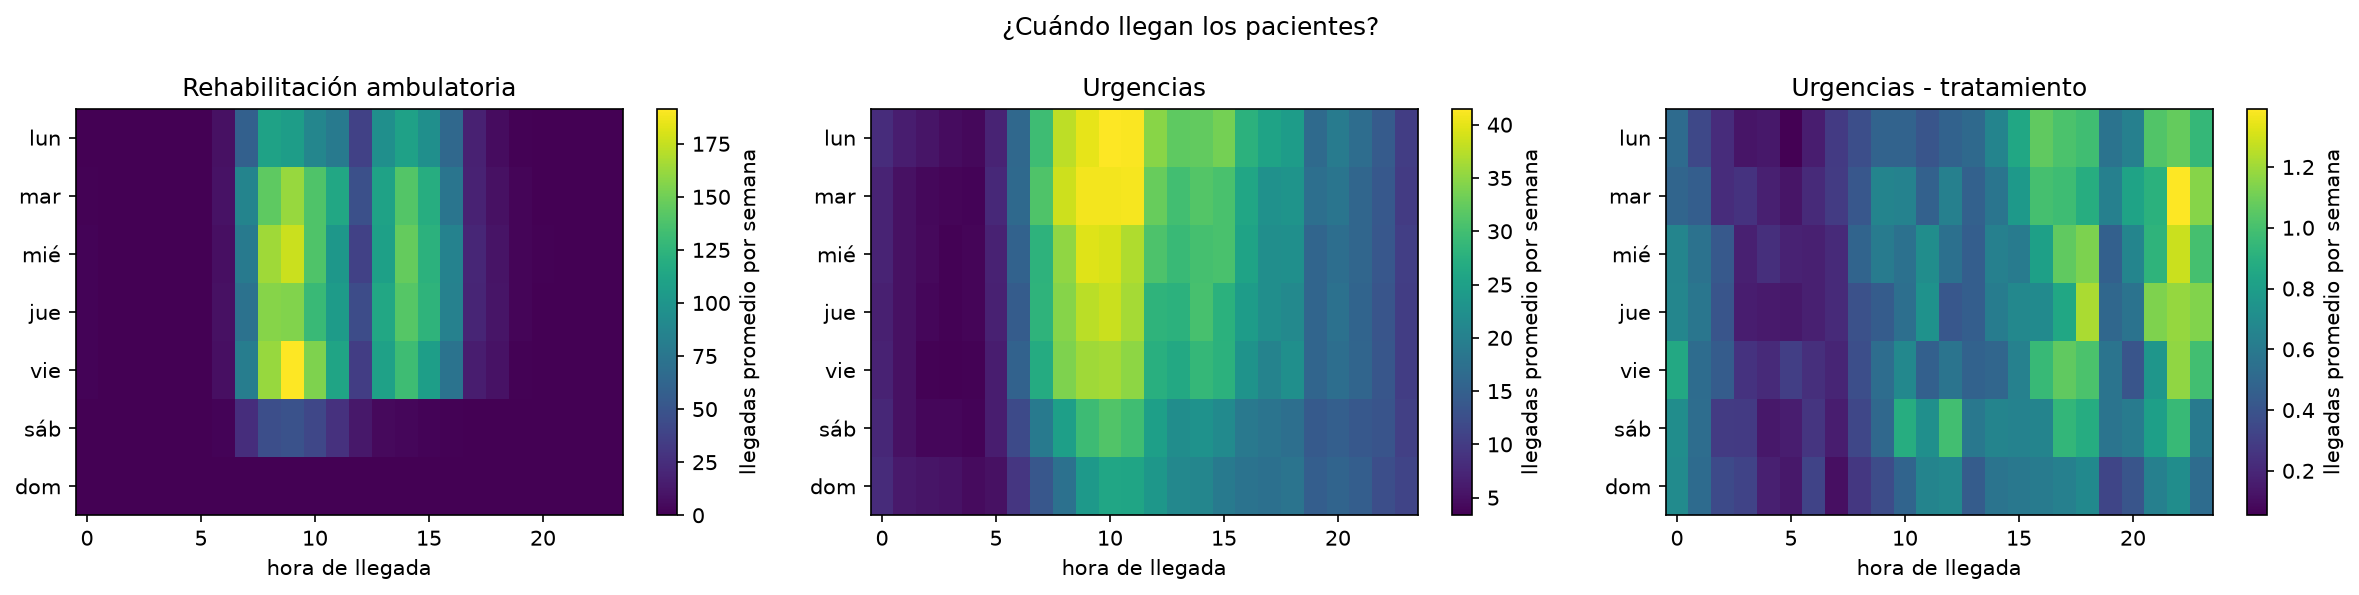
\includegraphics[width=0.96\textwidth]{01_llegadas_dia_hora.png}
\caption{Patrones descriptivos de llegadas promedio por hora y día de la semana (\protect\nolinkurl{01_llegadas_dia_hora.png}). Refleja distribución histórica archivada y no rendimiento predictivo.}
\label{fig:exploracion_llegadas}
\vspace{4pt}
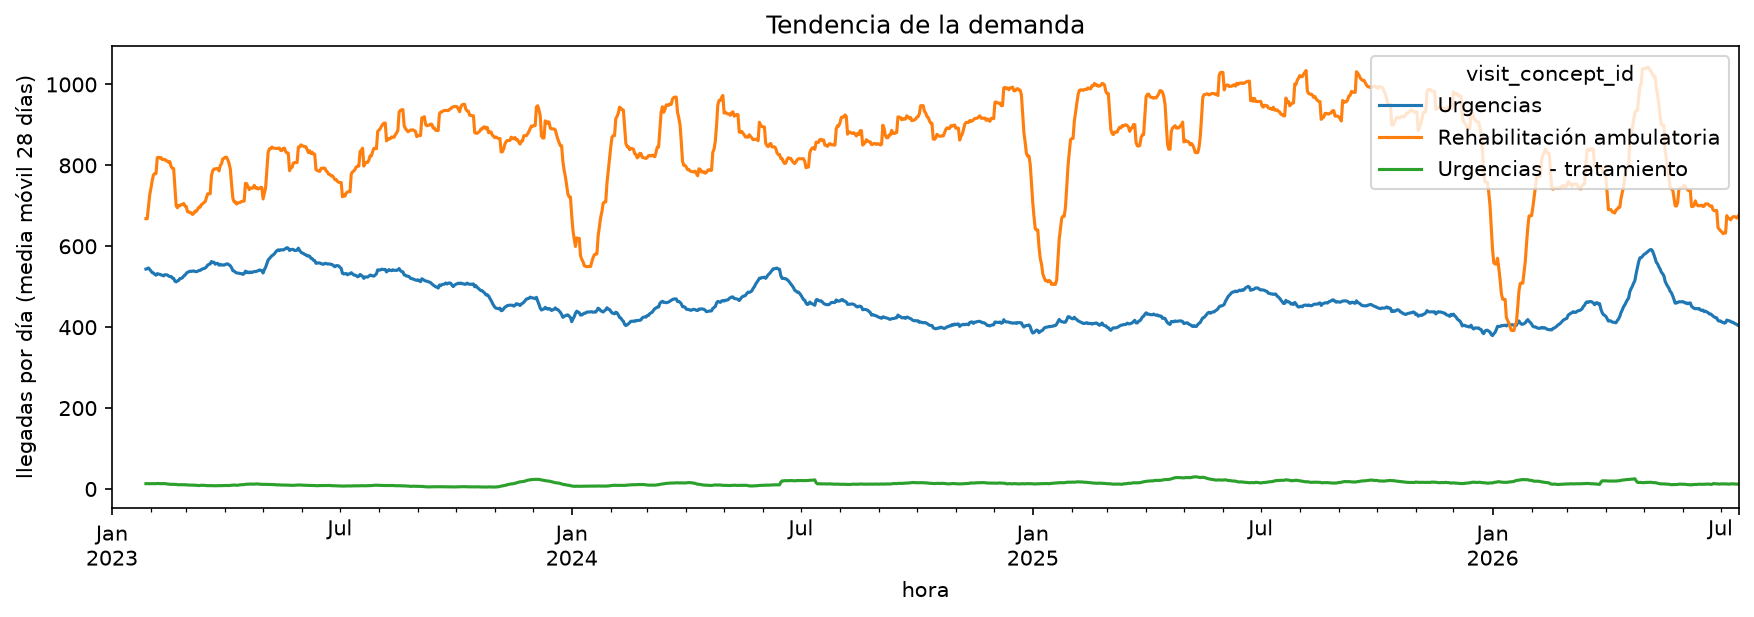
\includegraphics[width=0.96\textwidth]{02_tendencia.png}
\caption{Tendencia histórica de llegadas diarias en media móvil de 28 días, 2023--2026 (\protect\nolinkurl{02_tendencia.png}). Muestra descensos estacionales de Rehabilitación sin proyecciones fuera de muestra.}
\label{fig:exploracion_tendencia}
\vspace{4pt}
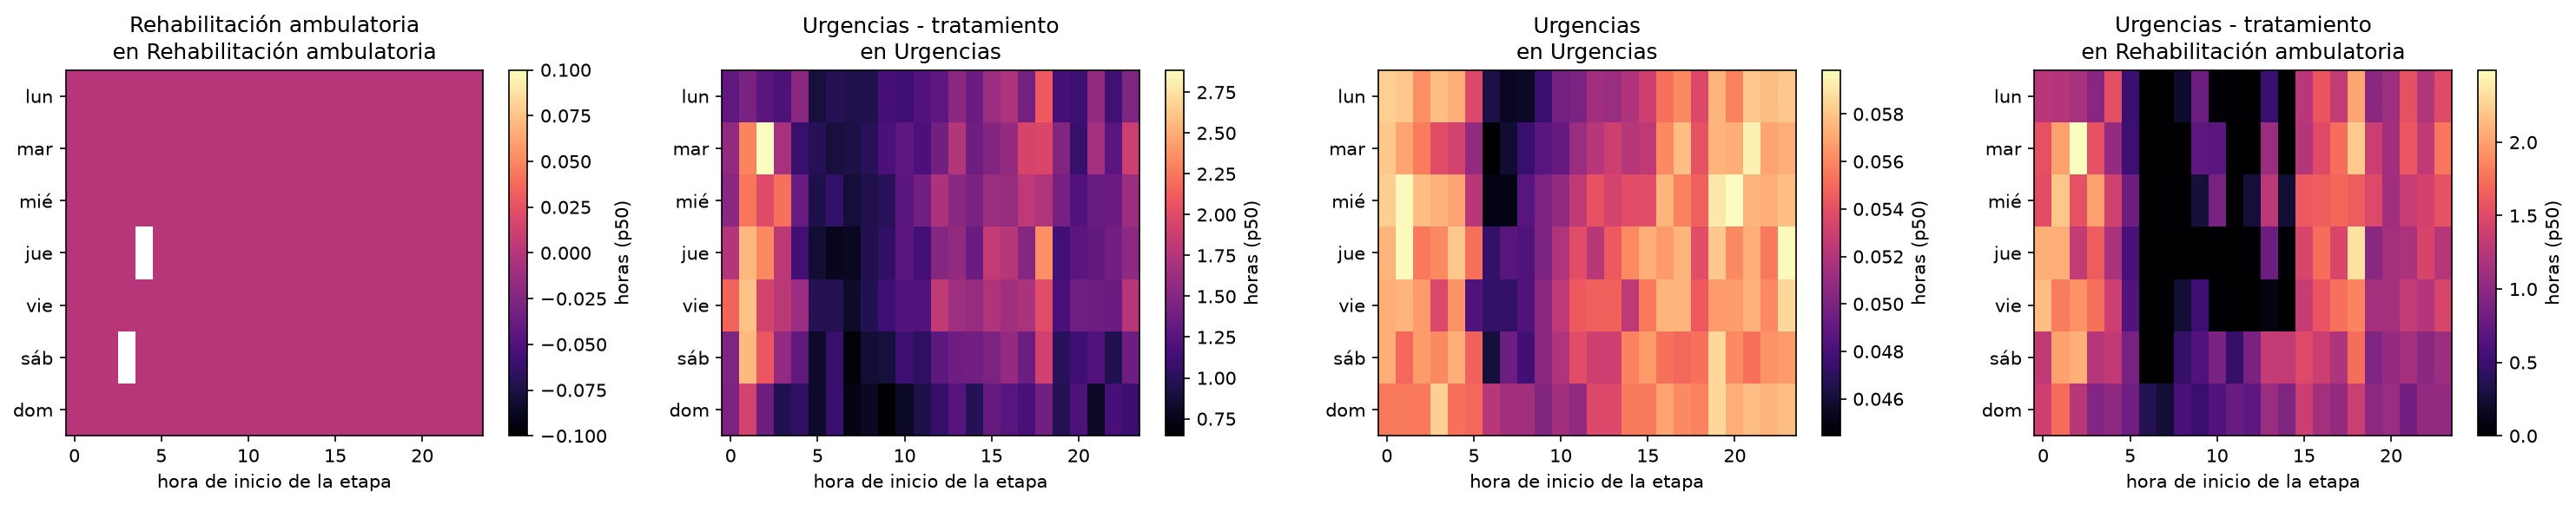
\includegraphics[width=0.96\textwidth]{03_duracion_etapas_franja.png}
\caption{Duración mediana (percentil 50) de etapas según día y hora de inicio (\protect\nolinkurl{03_duracion_etapas_franja.png}). Los valores nulos en Rehabilitación obedecen a ausencia de marcas de salida distintas del inicio.}
\label{fig:exploracion_duracion}
\end{figure*}

\subsection{Transición prioritaria entre Tratamiento Urgencias y Hospitalización}

La consulta \texttt{18\_transiciones\_etapas.sql} identifica como transición prioritaria el salto desde \textit{Treatment urgency} (\texttt{3045729}) hacia \textit{Inpatient Visit} (\texttt{9201}) dentro de visitas de Urgencias (\texttt{9203}), con \textbf{\num{47670} pasos}~\cite{mediflow2026optimizacion}. Con $\text{espera\_h} = \text{inicio\_siguiente} - \text{fin\_anterior}$, el $p_{50}$ mensual ponderado es \num{0,0}\,h y el $p_{90}$ mensual ponderado alcanza \textbf{\num{24,45}\,h} (\num{24,446}\,h sin redondear). Tres advertencias limitan su lectura: (1) admite valores negativos por solapamiento administrativo y no equivale a espera clínica por cama ni mide \textit{boarding}; (2) \num{24,45}\,h es el promedio mensual ponderado de $p_{90}$ y no el $p_{90}$ global de los \num{47670} registros agrupados; y (3) al cruzar mensualmente ese $p_{90}$ con el censo medio de Hospitalización surge una correlación ecológica negativa ($r = -0{,}481$; $p_{90}$ ponderado de \num{25,13}\,h en meses normales frente a \num{23,70}\,h en meses de censo alto)~\cite{mediflow2026optimizacion}, descartando una atribución causal simple a la congestión de piso sin auditar marcas en el HIS.

% Sección III: Calidad, preparación e integración de factores externos
% evidencia:E04,E05,E10,E26

\section{Calidad, preparación e integración de factores externos}

La confiabilidad predictiva y censal exige resolver anomalías administrativas previas en SQL y Python~\cite{mediflow2026calidad,mediflow2026informe}.

\subsection{Auditoría archivada de calidad y consistencia temporal}

La auditoría archivada del 28 de octubre de 2026~\cite{mediflow2026calidad} registró 0,00\,\% de nulos en columnas clave de \texttt{person} (\num{912205} filas), \texttt{visit\_occurrence} (\num{1706001}) y \texttt{visit\_detail} (\num{3281613}). Aunque las claves primarias no se repiten, agrupar por clave de evento reveló duplicidad administrativa en visitas principales y residual en etapas, junto con edades imposibles que distorsionaban el grupo pediátrico.

Para verificar si la anonimización desplazó fechas respecto del calendario colombiano, se midió el volumen relativo en festivos entre semana frente a tres semanas vecinas desplazando la referencia entre $-21$ y $+21$ días~\cite{mediflow2026calidad}. En Rehabilitación Ambulatoria (cierre no laboral), el mínimo global se produjo exactamente en desfase 0 días: volumen relativo de 0,0032 (0,32\,\%) en \texttt{visit\_occurrence} y 0,0033 (0,33\,\%) en \texttt{visit\_detail} (márgenes de 0,50 y 0,49 sobre el segundo menor desplazamiento), con caídas a 0,25\,\% y 0,21\,\% en lunes y martes de Carnaval. Urgencias mantiene operación continua (73,95\,\% en festivos). Esta prueba habilita variables calendáricas reales sin certificar exactitud horaria individual; todas las cifras provienen de registros archivados sin reejecución SQL.

\begin{table*}[t]
\caption{Reglas de calidad de datos, hallazgos archivados e implementación SQL vigente}
\label{tab:reglas_calidad}
\centering
\footnotesize
\begin{tabularx}{\textwidth}{@{}L{0.17\textwidth} L{0.31\textwidth} L{0.25\textwidth} Y@{}}
\toprule
Dimensión & Hallazgo archivado y población & Implementación vigente & Efecto o límite \\
\midrule
Nulos críticos & 0,00\,\% en claves y marcas de \texttt{person}, \texttt{visit\_occurrence} y \texttt{visit\_detail} & No requiere imputación de fechas & Completitud condicionada al extracto \\
Duplicados visitas & \num{228259} copias sobrantes (13,38\,\%) sobre \num{1706001} filas & \texttt{COUNT(DISTINCT (person\_id, concept, inicio))} en SQL \texttt{04}, \texttt{11}, \texttt{13} & Reduce llegadas totales a \num{1477742} ($-13{,}4\,\%$) \\
Duplicados etapas & \num{14081} copias sobrantes (0,43\,\%) sobre \num{3281613} etapas & Conteo agregado por etapa; tasa distinta a visitas & No extrapolar 0,43\,\% como tasa de visitas \\
Edades imposibles & 43 visitas (22 pacientes, 0,0025\,\%): edad $<0$ o $>110$ años & Etiqueta \texttt{invalida} en SQL \texttt{10} y \texttt{13} & Evita inflar el grupo pediátrico \texttt{0-17} \\
Etapas inválidas y huérfanas & 0\,\% sin fin o fin $<$ inicio; 117 huérfanas globales (91 en \texttt{9201}) & SQL \texttt{14}--\texttt{16}, \texttt{18} excluyen fechas inválidas; \texttt{SQL16} usa \texttt{LEFT JOIN} & Conserva huérfanas; contraste en recorte $p_{99{,}9}$ \\
Regularización & Ausencia de filas en horas o días sin movimientos & \texttt{grilla\_regular} rellena con 0 en \texttt{agregados.py} & Evita sesgar al alza promedios horarios/diarios \\
\bottomrule
\end{tabularx}
\ieeenota{Síntesis contrastada entre~\cite{mediflow2026calidad},~\cite{mediflow2026informe} (sec.~3) y los SQL \texttt{04}, \texttt{13}--\texttt{16} y \texttt{18} en \texttt{src/hun/data/sql/}.}
\end{table*}

\subsection{Depuración estadística de estancias extremas (\texorpdfstring{$p_{99{,}9}$}{p99.9}) y regla sobre huérfanas}

La auditoría sin recorte (\nolinkurl{23_duracion_etapas_percentiles.sql}) halló máximos crudos de \num{28070,3}\,h en Tratamiento Urgencias, \num{20730,3}\,h en Urgencias y \num{11213,6}\,h en Hospitalización~\cite{mediflow2026saturacion,mediflow2026informe}. Para evitar inflar la ocupación acumulada por cierres abiertos, las consultas \texttt{14}, \texttt{15} y \texttt{16} filtran por el percentil $p_{99{,}9}$ de cada etapa: \textbf{\num{1176,3}\,h} en Hospitalización (\num{1176,257222}\,h), \textbf{\num{283,7}\,h} en Tratamiento Urgencias, \textbf{\num{17,5}\,h} en Urgencias y \textbf{0,0\,h} en Rehabilitación~\cite{mediflow2026saturacion}.

En Hospitalización (\texttt{9201}), sobre \num{108601} etapas válidas se excluyen 107 superiores a \num{1176,3}\,h (todas con visita padre) y se conservan \textbf{\num{108494} etapas}, incluidas las 91 huérfanas ($<720$\,h)~\cite{mediflow2026informe}. Este filtro reduce $p_{50}/p_{75}/p_{90}$ poscalentamiento de 288 / 306 / 319 (máx. 378) a \textbf{283 / 297 / 309} (máx. \textbf{359}) en Hospitalización, y de 219 / 260 / 300 a \textbf{201 / 239 / 272} en Tratamiento Urgencias~\cite{mediflow2026informe}. Es un recorte estadístico agregado, no una adjudicación clínica. Asimismo, aunque pasajes previos de~\cite{mediflow2026calidad} recomendaban excluir huérfanas, la implementación vigente en \texttt{16\_duracion\_etapas\_diaria.sql} usa \texttt{LEFT JOIN visit\_occurrence} al igual que \texttt{SQL14} y \texttt{SQL15}, fijando la cohorte común de \num{108494} etapas (exigir visita padre reduciría la población a \num{108403}).

\subsection{Integración externa y protocolo de cuatro filtros}

El módulo \texttt{src/external/} construye \texttt{data/externos.parquet} integrando calendario colombiano (librería \texttt{holidays} con festivos, puentes y día posfestivo, Carnaval, Semana Santa, vacaciones y quincenas/primas), clima de Open-Meteo (Soledad) y SIVIGILA semanal (dengue e IRA grave con rezagos anti-fuga \texttt{lag2s} y \texttt{lag3s}). El control \texttt{data/externos\_fuentes.json} (27 de octubre de 2026) marca estado \texttt{ok} para calendario, clima (\texttt{2018-01-01} a \texttt{2026-10-21}) y epidemiología, sin implicar por sí solo aporte predictivo~\cite{mediflow2026informe}.

\begin{table*}[t]
\caption{Resultados archivados del protocolo de evaluación empírica de factores externos}
\label{tab:factores_externos}
\centering
\footnotesize
\begin{tabularx}{\textwidth}{@{}L{0.23\textwidth} l r r r r Y@{}}
\toprule
Grupo evaluado & Decisión & Mediana & Placebo & Pliegues & $p$-signo & Motivo registrado \\
\midrule
\texttt{festivos\_y\_puentes} & Acepta & $+33{,}80\,\%$ & $-1{,}80\,\%$ & 88\,\% & 0,000 & Cumple los 4 criterios \\
\texttt{carnaval\_y\_semana\_santa} & Acepta & $+3{,}49\,\%$ & $+1{,}26\,\%$ & 73\,\% & 0,014 & Cumple los 4 criterios \\
\texttt{vacaciones\_escolares} & Descarta & $+4{,}41\,\%$ & $-0{,}13\,\%$ & 65\,\% & 0,084 & $< 70\,\%$ de pliegues y $p > 0{,}05$ \\
\texttt{quincena\_y\_primas} & Descarta & $+1{,}17\,\%$ & $+0{,}79\,\%$ & 58\,\% & 0,279 & Placebo $> 0{,}5\times$, $< 70\,\%$ pliegues y $p > 0{,}05$ \\
\bottomrule
\end{tabularx}
\ieeenota{Fuente:~\cite{mediflow2026externos} (18 de noviembre de 2026, 26 pliegues \textit{walk-forward}). Criterios: mediana $\ge 1\,\%$, mejora en $\ge 70\,\%$ de pliegues, prueba unilateral de signo $p \le 0{,}05$ y placebo $< 0{,}5\times$ mejora real. \texttt{clima} y \texttt{epidemiologia} fueron descartados en una corrida inicial anterior~\cite{mediflow2026informe} y no tienen cifras en la tabla del 18 de noviembre. Las cifras de \texttt{docs/protocolo\_factores\_externos.md} ($+29{,}6\,\%$, placebo $-0{,}69\,\%$) corresponden a una corrida previa.}
\end{table*}

Cada grupo externo enfrenta cuatro filtros consecutivos sobre los 26 pliegues~\cite{mediflow2026externos}: ablación frente a base calendárica (día, mes, armónicos anuales), control de estacionalidad, prueba placebo desplazada y estabilidad/prueba de signo. Como resume la Tabla~\ref{tab:factores_externos}, solo \texttt{festivos\_y\_puentes} (6 variables) y \texttt{carnaval\_y\_semana\_santa} (5 variables) son aceptados en \texttt{lgbm\_final}.

% Sección IV: Metodología analítica y diseño de validación temporal
% evidencia:E08,E09,E11,E12,E13,E14

\section{Metodología analítica y diseño de validación temporal}

El diseño predictivo separa tres familias con fines distintos: una escalera experimental puntual (Poisson) para contrastar hipótesis y seleccionar externos; un conjunto cuantílico servido en la web para intervalos y explicabilidad; y un modelo sin rezagos cortos a cuatro meses. Todas prohíben particiones aleatorias y usan validación temporal de origen móvil (\textit{walk-forward})~\cite{hyndman_fpp3}.

\subsection{Validación temporal de origen móvil y política anti-fuga}

Para cada pliegue $k$ con origen $o_k$ y horizonte $h$, \texttt{src/hun/models/validacion.py} impone:
\begin{equation}
\label{eq:walk_forward}
\mathcal{D}_{\text{train}}^{(k)} = \{(s, t) : t < o_k\}, \quad
\mathcal{D}_{\text{test}}^{(k)} = \{(s, t) : o_k \le t < o_k + h\}.
\end{equation}
A corto plazo se emplean \textbf{26 pliegues} entre \texttt{2025-07-25} y \texttt{2026-07-10} con paso de 14 días y $h = 7$ días~\cite{mediflow2026demanda}. Al caer todos los orígenes en viernes, el día 1 del horizonte es siempre viernes y el día 7 jueves; día de horizonte y día de semana quedan confundidos. A largo plazo se usan \textbf{13 pliegues} entre \texttt{2025-03-24} y \texttt{2026-03-19} con paso de 30 días y $h = 120$ días, generando ventanas ampliamente solapadas y no independientes~\cite{mediflow2026largoplazo}.

En \texttt{construir\_features\_demanda} (\texttt{demanda.py}), el objetivo $y_{s,t}$ se enmascara para $t \ge o_k$ antes de calcular rezagos semanales (\texttt{llegadas\_lag\_7} a \texttt{56}, \texttt{rezago\_prom\_4s} y \texttt{rezago\_mediana\_8s}), garantizando que el horizonte $[o_k, o_k+7\,\text{d})$ consulte solo historia previa a $o_k$. SIVIGILA usa rezagos de 2--3 semanas y largo plazo reemplaza clima futuro por medianas históricas previas al corte. Como límite, esta garantía del backtest 1--7 días no se extiende automáticamente cuando la web consulta fechas poscorte con \texttt{medianas\_dw} ni al consultar historia ya vista por el modelo final~\cite{mediflow2026bundle,mediflow2026informe}.

\subsection{Métricas de evaluación y techo Poisson idealizado}

Ante días con conteo nulo o bajo (evitando divergencias del MAPE), la decisión \texttt{DEC-003} adopta WAPE, MAE, RMSE, sesgo y cobertura empírica (excluyendo la serie residual \texttt{Otros}):
\begin{equation}
\label{eq:metricas}
\begin{gathered}
\text{WAPE} = \frac{\sum_{i=1}^{n} |y_i - \hat{y}_i|}{\sum_{i=1}^{n} |y_i|}, \quad
\text{Exactitud} = 1 - \text{WAPE}, \\
\text{MAE} = \frac{1}{n}\sum_{i=1}^{n} |y_i - \hat{y}_i|, \quad
\text{Sesgo} = \frac{1}{n}\sum_{i=1}^{n} (\hat{y}_i - y_i), \\
\text{RMSE} = \sqrt{\frac{1}{n}\sum_{i=1}^{n} (y_i - \hat{y}_i)^2}, \\
\text{Cob.} = \frac{1}{n}\sum_{i=1}^{n} \mathbf{1}\!\left\{\hat{q}_{0{,}10,i} \le y_i \le \hat{q}_{0{,}90,i}\right\}.
\end{gathered}
\end{equation}
Aquí «exactitud» denota estrictamente $1-\text{WAPE}$, un sesgo positivo indica sobreestimación promedio y la meta de 80\,\% es criterio interno del equipo, no requisito de~\cite{hun2026terminos,mediflow2026demanda}. Para series de bajo volumen (como Tratamiento Urgencias, $\approx 15{,}2$/día), \texttt{techo\_exactitud\_poisson} calcula un techo optimista con $X \sim \text{Poisson}(\mu)$, $\mu = \bar{y}\cdot d$ ($d \in \{1,7\}$):
\begin{equation}
\label{eq:techo_poisson}
\text{Techo}(\mu) = 1 - \frac{\mathbb{E}\bigl[|X - \mu|\bigr]}{\mu},
\end{equation}
asumiendo tasa verdadera conocida y ruido puro sin deriva semanal~\cite{mediflow2026demanda}.

\subsection{Familia experimental puntual (escalera Poisson y LightGBM)}

En \texttt{src/hun/models/demanda.py} se comparan cuatro escalones sobre los 26 pliegues: (1) \texttt{linea\_base} (mediana del mismo día en las últimas 8 semanas); (2) \texttt{poisson\_calendario} (\texttt{PoissonRegressor}, $\alpha=10^{-4}$) ajustado de forma estratificada por servicio; (3) \texttt{lgbm\_todos\_externos} con LightGBM~\cite{ke2017lightgbm} y pérdida Poisson (\texttt{n\_estimators=200}, \texttt{learning\_rate=0.05}, \texttt{num\_leaves=15}, \texttt{min\_child\_samples=15}); y (4) \texttt{lgbm\_final}, restringido a externos aprobados. Los escalones LightGBM añaden ponderación exponencial $w_i = 0{,}5^{\text{edad}_i / 180}$ (vida media 180 días) y corrección de nivel local en \texttt{ajustar\_predecir\_lgbm\_nivel} vía \texttt{init\_score} $= \log(\max(\text{rezago\_mediana\_8s},\,0{,}5))$, prediciendo multiplicadores logarítmicos sobre el nivel reciente.

\subsection{Familia cuantílica servida en la aplicación web}

El paquete \texttt{models/modelos\_web\_bundle.joblib} (\texttt{v2.0}) no sirve \texttt{lgbm\_final}. En \texttt{explicacion.py}, tres regresores LightGBM independientes ajustan cuantiles $\tau \in \{0{,}10,\, 0{,}50,\, 0{,}90\}$ bajo pérdida \textit{pinball}~\cite{koenker1978quantiles,ke2017lightgbm}:
\begin{equation}
\label{eq:pinball}
\rho_\tau(u) = u\bigl(\tau - \mathbf{1}\{u < 0\}\bigr), \qquad u = y - \hat{q}_\tau(x),
\end{equation}
con ordenamiento monotónico y truncamiento en cero:
\begin{equation}
\label{eq:orden_cuantiles}
(\tilde{q}_{0{,}10}, \tilde{q}_{0{,}50}, \tilde{q}_{0{,}90}) = \max\bigl(0,\operatorname{sort}(\hat{q}_{0{,}10}, \hat{q}_{0{,}50}, \hat{q}_{0{,}90})\bigr),
\end{equation}
lo cual garantiza coherencia ordinal sin calibrar cobertura. La mediana $\hat{q}_{0{,}50}$ se explica mediante valores SHAP exactos (\texttt{TreeExplainer})~\cite{lundberg2017shap}:
\begin{equation}
\label{eq:shap}
f(x) = \phi_0 + \sum_{j=1}^{M} \phi_j(x),
\end{equation}
midiendo contribuciones marginales no causales al pronóstico. La inspección de \texttt{entrenar\_modelos\_cuantiles} y de \texttt{cols} en el bundle \texttt{v2.0} confirma que esta familia \textbf{no} usa \texttt{init\_score} ni pesos por recencia, y sus 21 variables (5 de calendario, 10 de rezago y 6 de \texttt{festivos\_y\_puentes}) omiten las 5 de \texttt{carnaval\_y\_semana\_santa}~\cite{mediflow2026bundle}.

\subsection{Modelo independiente de horizonte extendido}

Para proyectar agosto--noviembre de 2026 más allá de \texttt{2026-07-16}, \texttt{src/hun/models/largo\_plazo.py} entrena un LightGBM Poisson con recencia (180 días, \texttt{min\_child\_samples=20}) sin rezagos cortos, usando 7 variables de calendario, 6 de \texttt{festivos\_y\_puentes}, \texttt{tendencia\_anios}, servicio y medianas climáticas previas al corte. Los intervalos parten de regresores en $p_{05}$ y $p_{95}$ (\texttt{CUANTIL\_BAJO=0,05}, \texttt{CUANTIL\_ALTO=0,95}) escalados alrededor de $\hat{y}$ según el mes $m \in \{1..4\}$ por $1 + 0{,}10\,(m-1)$, aunque el JSON los rotule como \texttt{min\_diario}/\texttt{max\_diario} o $[p_{10}, p_{90}]$~\cite{mediflow2026largoplazo}.

% Sección V: Resultados predictivos por familia de evidencia
% evidencia:E08,E09,E12,E13,E14

\section{Resultados predictivos por familia de evidencia}

Los resultados predictivos se presentan en tres bloques independientes: la corrida puntual del 18 de noviembre de 2026, los metadatos inspeccionados del artefacto cuantílico servido (\texttt{v2.0}) frente al reporte histórico del 3 de noviembre, y las dos corridas comprobadas a 120 días.

\subsection{Experimento puntual Poisson: escalera, servicios y estabilidad}

En los 26 pliegues \textit{walk-forward} reportados el 18 de noviembre de 2026~\cite{mediflow2026demanda}, incorporar estratificación por servicio, nivel local con pesos por recencia y externos aprobados reduce el error global de forma sostenida (Tabla~\ref{tab:escalera_poisson}).

\begin{table}[htbp]
\caption{Escalera predictiva puntual en 26 pliegues \textit{walk-forward} (18 de noviembre de 2026)}
\label{tab:escalera_poisson}
\centering
\scriptsize
\begin{tabularx}{\columnwidth}{@{}Y r r r r r@{}}
\toprule
Modelo evaluado & WAPE & MAE & RMSE & Sesgo & Mej. rel. \\
\midrule
1. Línea base (8 sem.) & 18,0\,\% & 77,02 & 201,34 & $+21{,}44$ & Ref. \\
2. Poisson estratificado & 15,6\,\% & 66,86 & 125,91 & $+6{,}41$ & $+13{,}2\,\%$ \\
3. LGBM nivel local (todos) & 10,5\,\% & 44,84 & 83,82 & $-6{,}00$ & $+41{,}8\,\%$ \\
4. LGBM final (\texttt{lgbm\_final}) & 10,5\,\% & 44,94 & 83,67 & $-5{,}70$ & $+41{,}6\,\%$ \\
\bottomrule
\end{tabularx}
\ieeenota{Datos archivados de~\cite{mediflow2026demanda} (sec.~1, orígenes \texttt{2025-07-25} a \texttt{2026-07-10}, horizonte 1--7\,d, sin \texttt{Otros}). Las mejoras relativas fueron calculadas con cifras sin redondear. \texttt{lgbm\_final} conserva solo \texttt{festivos\_y\_puentes} y \texttt{carnaval\_y\_semana\_santa}.}
\end{table}

El desempeño desagregado de \texttt{lgbm\_final} muestra marcada heterogeneidad (Tabla~\ref{tab:servicios_poisson}). Urgencias (\texttt{9203}) y Rehabilitación (\texttt{581479}) obtienen WAPE de 8,4\,\% y 11,0\,\% (exactitudes $1-\text{WAPE}$ de 91,6\,\% y 89,0\,\%); sin embargo, en Rehabilitación la exactitud cae a 51,3\,\% los sábados (87,1 llegadas/día) y 15,6\,\% los domingos (2,2/día), frente a 85,6\,\%--90,9\,\% de lunes a viernes (835,7--1.306,2/día)~\cite{mediflow2026demanda}. En Tratamiento Urgencias (\texttt{3045729}, media 15,17/día), el WAPE diario alcanza 43,5\,\% (exactitud 56,5\,\%, MAE 6,59), frente a un techo Poisson idealizado de 79,5\,\% diario; al agregar la semana completa alcanza 77,0\,\% frente a un techo semanal de 92,3\,\%~\cite{mediflow2026demanda}. Al quedar bajo ambas cotas, influyen tanto la varianza de conteos bajos como cambios semanales de tasa.

\begin{table}[htbp]
\caption{Desempeño por servicio del experimento puntual \texttt{lgbm\_final}}
\label{tab:servicios_poisson}
\centering
\scriptsize
\begin{tabularx}{\columnwidth}{@{}Y r r r r r@{}}
\toprule
Servicio & WAPE & $1-\text{WAPE}$ & MAE & Sesgo & Prom. \\
\midrule
Urgencias (\texttt{9203}) & 8,4\,\% & 91,6\,\% & 37,02 & $-7{,}83$ & 443,16 \\
Rehabilitación (\texttt{581479}) & 11,0\,\% & 89,0\,\% & 91,22 & $-10{,}12$ & 826,54 \\
Trat. Urgencias (\texttt{3045729}) & 43,5\,\% & 56,5\,\% & 6,59 & $+0{,}86$ & 15,17 \\
\bottomrule
\end{tabularx}
\ieeenota{Datos archivados de~\cite{mediflow2026demanda} (sec.~2, 26 pliegues, 182 días/servicio, sin \texttt{Otros}). No transferir estas cifras al modelo cuantílico web.}
\end{table}

En días normales, el WAPE baja de 12,4\,\% en línea base (MAE 55,63; sesgo $-3{,}45$) a 10,3\,\% en \texttt{lgbm\_final} (MAE 45,97; sesgo $-6{,}96$); en festivos, cae de 317,8\,\% (MAE 409,64; sesgo $+408{,}36$, por sobreestimación en cierres de Rehabilitación) a 22,5\,\% (MAE 29,03; sesgo $+13{,}89$)~\cite{mediflow2026demanda}. A lo largo del horizonte 1--7 días, el WAPE oscila entre 9,4\,\% (día 7, jueves) y 17,0\,\% (día 2, sábado), y entre pliegues va de 5,4\,\% (pliegue 17, \texttt{2026-03-20}) a 28,0\,\% en el pliegue 11 (\texttt{2025-12-26}, fin de año; línea base 137,9\,\%) y 27,6\,\% en el pliegue 19 (\texttt{2026-04-17})~\cite{mediflow2026demanda} (detalle completo en Anexo~B).

\subsection{Artefacto cuantílico servido en la aplicación web (\texttt{v2.0})}

Los metadatos inspeccionados directamente en \texttt{models/modelos\_web\_bundle.joblib} (\texttt{comparacion\_real} sobre 182 días, \texttt{2025-07-25} a \texttt{2026-07-16}) reportan el rendimiento del modelo cuantílico $p_{10}/p_{50}/p_{90}$ servido por la API (Tabla~\ref{tab:bundle_cuantilico}). El WAPE de $p_{50}$ es 8,91\,\% en Urgencias, 11,08\,\% en Rehabilitación y 42,18\,\% en Tratamiento Urgencias; las coberturas $p_{10}$--$p_{90}$ (78,57\,\%, 64,29\,\% y 73,08\,\%) quedan por debajo de 80\,\%, especialmente en Rehabilitación por sus cierres bruscos y la ausencia de nivel local.

\begin{table*}[t]
\caption{Métricas archivadas del modelo cuantílico servido en el artefacto web \texttt{v2.0}}
\label{tab:bundle_cuantilico}
\centering
\footnotesize
\begin{tabularx}{\textwidth}{@{}Y r r r r r r@{}}
\toprule
Servicio en bundle \texttt{v2.0} & WAPE & MAE & RMSE & Sesgo & Cob. $p_{10}$--$p_{90}$ & Exact. sem. \\
\midrule
Urgencias (\texttt{9203}) & 8,91\,\% & 39,50 & 53,82 & $-2{,}69$ & 78,57\,\% & 94,75\,\% \\
Rehabilitación (\texttt{581479}) & 11,08\,\% & 91,55 & 137,57 & $+4{,}22$ & 64,29\,\% & 91,63\,\% \\
Tratamiento Urg. (\texttt{3045729}) & 42,18\,\% & 6,40 & 8,47 & $-0{,}64$ & 73,08\,\% & 76,60\,\% \\
\bottomrule
\end{tabularx}
\ieeenota{Metadatos de \texttt{comparacion\_real} en~\cite{mediflow2026bundle} (182 días: \texttt{2025-07-25} a \texttt{2026-07-16}, corte exclusivo \texttt{2026-07-17}; vía \texttt{GET /api/modelo}). Cobertura calculada antes de redondear puntos a enteros. Techos Poisson almacenados: Urgencias 96,21\,\% diario / 98,57\,\% semanal; Rehabilitación 97,22\,\% / 98,95\,\%; Tratamiento Urgencias 79,53\,\% / 92,26\,\%.}
\end{table*}

Estas cifras no deben confundirse con el reporte histórico del 3 de noviembre de 2026~\cite{mediflow2026intervalos}, que documentó cobertura global de 83,2\,\% (85,2\,\% en Urgencias, 72,0\,\% en Rehabilitación, 75,8\,\% en Tratamiento y 100,0\,\% en \texttt{Otros}; amplitud media 112,6 pacientes) sobre una versión previa e incluyendo \texttt{Otros}. Además, al consultar fechas futuras sin rezagos observados, \texttt{predict.py} usa \texttt{medianas\_dw}, lo cual no replica las condiciones del backtest 1--7 días. La Fig.~\ref{fig:resumen_escalera} separa visualmente el experimento puntual de la simulación de altas tempranas.

\begin{figure*}[t]
\centering
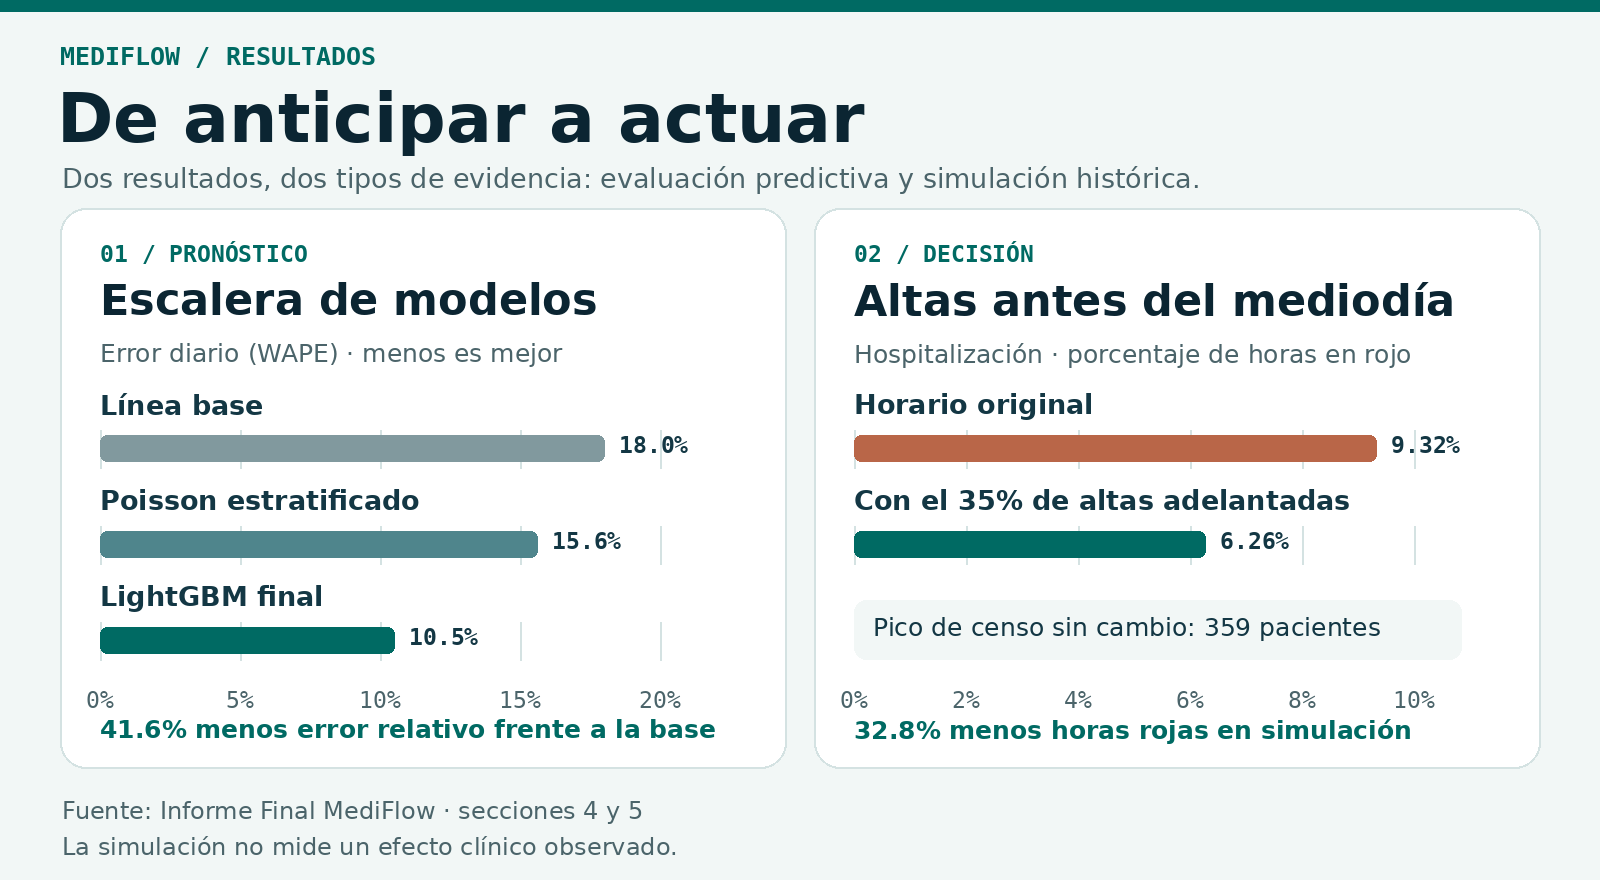
\includegraphics[width=0.84\textwidth]{resumen_escalera_optimizacion.png}
\caption{Síntesis comparativa entre evaluación predictiva puntual y simulación histórica de altas (\texttt{resumen\_escalera\_optimizacion.png}). Panel izquierdo: experimento puntual Poisson en 26 pliegues (no modelo cuantílico web). Panel derecho: simulación determinista de adelanto del 35\,\% de altas en Hospitalización (no ensayo clínico).}
\label{fig:resumen_escalera}
\end{figure*}

\subsection{Horizonte extendido a cuatro meses: reporte histórico frente a bundle}

Se documenta por separado la divergencia entre el reporte histórico del 3 de noviembre de 2026~\cite{mediflow2026largoplazo} y el campo \texttt{largo\_plazo} inspeccionado en el bundle \texttt{v2.0}~\cite{mediflow2026bundle} (Tabla~\ref{tab:largo_plazo_comparado}). En~\cite{mediflow2026largoplazo}, la exactitud global cae de 87,8\,\% en el mes 1 (WAPE 12,2\,\%) a 86,6\,\% (13,4\,\%), 83,5\,\% (16,5\,\%) y 78,7\,\% en el mes 4 (WAPE 21,3\,\%, ancho medio 424,5 pacientes), con 50,7\,\% de exactitud semanal (WAPE 49,3\,\%) en Tratamiento Urgencias. En el bundle \texttt{v2.0}, las tres series muestran menor WAPE y proyecciones agosto--noviembre coherentes con los niveles recientes de mediados de 2026 (frente a los promedios menores de la corrida del 3 de noviembre), aunque Rehabilitación cae bajo 80\,\% de cobertura en el mes 1 (77,69\,\%). El desglose mensual completo figura en el Anexo~B.

\begin{table*}[t]
\caption{Desempeño del modelo de largo plazo (120 días, 13 pliegues): reporte archivado frente a bundle servido}
\label{tab:largo_plazo_comparado}
\centering
\footnotesize
\begin{tabularx}{\textwidth}{@{}L{0.25\textwidth} Y r r r r r@{}}
\toprule
Fuente y corrida & Servicio & WAPE & $1-\text{WAPE}$ & MAE & Sesgo & Cobertura \\
\midrule
Reporte archivado & Global (sin \texttt{Otros}) & 15,7\,\% & 84,3\,\% & 57,9 & --- & 86,5\,\% \\
(\texttt{2026-11-03})~\cite{mediflow2026largoplazo} & Urgencias (\texttt{9203}) & 14,0\,\% & 86,0\,\% & 52,3 & $+20{,}1$ & 85,4\,\% \\
 & Rehabilitación (\texttt{581479}) & 15,5\,\% & 84,5\,\% & 111,7 & $+44{,}2$ & 85,3\,\% \\
 & Tratamiento (\texttt{3045729}) & 64,4\,\% & 35,6\,\% & 9,8 & $+4{,}9$ & 88,7\,\% \\
\midrule
Bundle servido \texttt{v2.0} & Urgencias (\texttt{9203}) & 11,63\,\% & 88,4\,\% & 51,8 & $-15{,}1$ & 87,18\,\% \\
(inspección \texttt{2026-11-19})~\cite{mediflow2026bundle} & Rehabilitación (\texttt{581479}) & 14,33\,\% & 85,7\,\% & 122,7 & $-2{,}9$ & 83,40\,\% \\
 & Tratamiento (\texttt{3045729}) & 58,12\,\% & 41,9\,\% & 10,1 & $+3{,}9$ & 88,65\,\% \\
\bottomrule
\end{tabularx}
\ieeenota{Dos corridas independientes sobre 13 pliegues solapados (\texttt{2025-03-24} a \texttt{2026-03-19}). En~\cite{mediflow2026largoplazo} las proyecciones ago--nov 2026 promedian 215,7--221,0/d (Urgencias) y 330,5--385,9/d (Rehabilitación); en~\cite{mediflow2026bundle}, promedian 415,6--433,2/d (Urgencias), 661,5--789,6/d (Rehabilitación, cobertura 77,69\,\% mes 1 y 81,79\,\%--87,95\,\% meses 2--4) y 15,6--16,1/d (Tratamiento). Son extrapolaciones desde el corte de julio de 2026, no demanda real observada.}
\end{table*}

% Sección VI: Optimización operacional y simulaciones paramétricas
% evidencia:E15,E16,E17,E18,E19,E20

\section{Optimización operacional y simulaciones paramétricas}

La capa de decisión integra tres modelos analíticos: colas M/M/$c$ (Erlang~C), Ley de Little y simulación horaria de altas tempranas~\cite{mediflow2026optimizacion,mediflow2026informe}. Todas las cifras expresan escenarios históricos o paramétricos condicionados a supuestos explícitos, nunca dotación contractual ni impacto clínico observado~\cite{green2006queueing}.

\subsection{Dimensionamiento paramétrico con Erlang~C}

En \texttt{src/hun/models/optimizacion.py}, cada franja de 6\,h se modela como cola M/M/$c$ con llegadas de Poisson de tasa horaria $\lambda$ (grilla regular con ceros dividida entre 6\,h), atención exponencial de media supuesta $1/\mu \in \{15,\,20,\,30\}\,\text{min}$ ($\mu = 60/t_{\text{serv}}$ pac./h), cola única y sin abandono~\cite{green2006queueing,mediflow2026optimizacion}. Cada servidor $c$ denota un \textbf{equipo activo equivalente}, no una plaza contractual. Con $a = \lambda/\mu$ y $\rho = \lambda/(c\mu)$, el algoritmo calcula Erlang~B por recurrencia estable ($B_0=1$, $B_k = a B_{k-1}/(k + a B_{k-1})$) y obtiene para $\rho < 1$:
\begin{equation}
\label{eq:erlang_c}
C(c, a) = \frac{B_c}{1 - \rho + \rho B_c}, \qquad
W_q = \frac{60 \cdot C(c, a)}{c\mu - \lambda},
\end{equation}
donde $W_q$ es la espera media en minutos (si $\rho \ge 1$ la cola es inestable)~\cite{mediflow2026optimizacion}. Se elige el menor entero $c \ge \lfloor a \rfloor + 1$ con $W_q < 15\,\text{min}$ y $P(\text{espera} \le 15\,\text{min}) = 1 - C(c,a)\exp(-(c\mu - \lambda)\cdot 15/60) \ge 0{,}80$. En franjas pico (Tabla~\ref{tab:erlang_sensibilidad}), Urgencias (06--12\,h, 20\,min) pasa de 12 a 15 equipos equivalentes bajo demanda $p_{90}$ (espera media 6,094\,min) y Rehabilitación (06--12\,h, 30\,min) de 42 a 70 (5,303\,min). La alta sensibilidad frente a $1/\mu$ (12--22 en Urgencias $p_{90}$; 35--70 en Rehabilitación $p_{90}$) exige medir tiempos clínicos reales antes de decidir dotación.

\begin{table*}[t]
\caption{Dimensionamiento Erlang~C en franja pico y sensibilidad al supuesto de tiempo de atención}
\label{tab:erlang_sensibilidad}
\centering
\footnotesize
\begin{tabularx}{\textwidth}{@{}Y r r r r r L{0.18\textwidth}@{}}
\toprule
Servicio y franja pico & $1/\mu$ (min) & $\lambda_{\text{norm}}$/h & $\lambda_{p90}$/h & $c_{\text{norm}}$ & $c_{p90}$ & Espera media en $p_{90}$ (min) \\
\midrule
Urgencias $\cdot$ 06--12\,h (base) & 20 & 29,250 & 39,667 & 12 & 15 & 6,094 \\
Urgencias $\cdot$ 06--12\,h (sens.) & 15 / 30 & 29,250 & 39,667 & 9 / 17 & 12 / 22 & $\Delta_{p90} = 3 / 5$ eq. \\
Rehabilitación $\cdot$ 06--12\,h (base) & 30 & 77,584 & 133,333 & 42 & 70 & 5,303 \\
Rehabilitación $\cdot$ 06--12\,h (sens.) & 15 / 20 & 77,584 & 133,333 & 21 / 28 & 35 / 47 & $\Delta_{p90} = 14 / 19$ eq. \\
Tratamiento Urg. $\cdot$ 18--24\,h (base) & 20 & 0,819 & 1,667 & 1 & 2 & 1,672 \\
Tratamiento Urg. $\cdot$ 18--24\,h (sens.) & 15 / 30 & 0,819 & 1,667 & 1 / 2 & 2 / 2 & $\Delta_{p90} = 1 / 0$ eq. \\
\bottomrule
\end{tabularx}
\ieeenota{Datos archivados de~\cite{mediflow2026optimizacion}. $1/\mu$ es un supuesto paramétrico y la espera reportada es el promedio esperado bajo tasa $p_{90}$, no el percentil 90 de espera del paciente. El detalle de las 12 franjas figura en el Anexo~B.}
\end{table*}

\subsection{Ley de Little en Hospitalización y contraste entre poblaciones}

La Ley de Little~\cite{little1961} vincula en régimen estacionario el censo medio $L$, la tasa de llegada $\lambda$ (ingresos/día) y la permanencia media $W$ (horas) sobre población y ventana consistentes:
\begin{equation}
\label{eq:little}
L = \frac{\lambda \cdot W}{24},
\end{equation}
sin intercambiar medias con medianas ni mezclar cohortes~\cite{mediflow2026informe} (Tabla~\ref{tab:little_poblaciones}). En la cohorte alineada filtrada por $p_{99{,}9}$ (\texttt{sql14\_15\_16\_p999}, \num{108494} etapas), $L = \text{\num{277,52}}$ pacientes concuerda con el censo medio horario de \textbf{\num{277,47}} pacientes en 1.294 días (\num{278,61} poscalentamiento; mediana 283,0). El bundle \texttt{v2.0} conserva en cambio una referencia híbrida de \textbf{\num{284,01} pacientes} (tasa $p_{99{,}9}$ de \num{83,843895}/día combinada con duración previa sin recorte y con visita padre $W = \text{\num{81,297108}}$\,h). Sobre esa referencia del bundle, acortar $W$ en 2, 4, 6 y 8\,h equivale teóricamente a \num{6,987} (2,460\,\%), \num{13,974} (4,920\,\%), \num{20,961} (7,380\,\%) y \num{27,948} (9,840\,\%) camas medias equivalentes~\cite{mediflow2026optimizacion,mediflow2026bundle}: específicamente, $-4$\,h libera \textbf{\num{13,97} camas medias equivalentes} (4,92\,\%), sin constituir expansión física ni ahorro garantizado.

\begin{table*}[t]
\caption{Contraste de Ley de Little por población y ventana temporal en Hospitalización (\texttt{9201})}
\label{tab:little_poblaciones}
\centering
\footnotesize
\begin{tabularx}{\textwidth}{@{}Y r r r r R{2.3cm} R{1.45cm}@{}}
\toprule
Régimen / población & Etapas $E,S$ / $W$ & $\lambda$ (/d) & $W$ (h) & $\lambda W/24$ & Media hor. (1.294\,d / +24\,d) & Mediana (+24\,d) \\
\midrule
\nolinkurl{sql14_15_16_p999} (con huérfanas) & \num{108494} / \num{108494} & 83,843895 & 79,438491 & 277,52 & 277,47 / 278,61 & 283,0 \\
\nolinkurl{padre_y_p999} (exige visita padre) & \num{108403} / \num{108403} & 83,773570 & 79,428945 & 277,25 & 277,20 / 278,60 & --- \\
Híbrido bundle \texttt{v2.0} & \num{108494} / \num{108510} & 83,843895 & 81,297108 & 284,01 & --- & --- \\
Bruta sin recorte (con huérfanas) & \num{108601} / \num{108601} & 83,926584 & 81,305079 & 284,32 & 284,27 / 285,54 & 288,0 \\
\bottomrule
\end{tabularx}
\ieeenota{Verificación documentada en PostgreSQL~\cite{mediflow2026informe} (sec.~3) y metadatos de~\cite{mediflow2026bundle}. Productos exactos: \num{277,5177}, \num{277,2514}, \num{284,0111} y \num{284,3191} pac. Para \texttt{sql14\_15\_16\_p999}, la media continua en 1.294\,d (31.056\,h hasta \texttt{2026-07-18 00:00}) es \num{277,4669}, frente a \num{277,4644} hasta última salida (31.062\,h) y \num{278,6203} tras calentamiento (30.483\,h). La mediana no contrasta Little.}
\end{table*}

\subsection{Simulación horaria de rondas de alta temprana}

En \texttt{calcular\_ley\_little\_y\_altas\_tempranas}, una fracción $p \in \{20\,\%, 35\,\%, 50\,\%\}$ de las salidas vespertinas en $[14{:}00, 20{:}00)$ se traslada uniformemente a $[08{:}00, 12{:}00)$ del mismo día con umbral rojo fijo $>309$, midiendo la variación en puntos porcentuales y relativa:
\begin{equation}
\label{eq:reduccion_rojas}
\Delta_{\text{pp}} = H_{\text{base}} - H_{\text{sim}}(p), \qquad
\Delta_{\text{rel}} = 100 \cdot \frac{H_{\text{base}} - H_{\text{sim}}(p)}{H_{\text{base}}}.
\end{equation}
Como muestra la Tabla~\ref{tab:altas_tempranas}, adelantar el \textbf{35\,\%} reduce las horas en alerta roja de 9,32\,\% a 6,26\,\% ($-3{,}06$\,pp; $-32{,}8\,\%$ relativo), manteniendo intacto el pico máximo histórico en \textbf{359 pacientes}. En la API, valores intermedios del deslizador se interpolan linealmente entre $\{0, 20, 35, 50, 100\}$ vía \texttt{numpy.interp}~\cite{mediflow2026optimizacion}.

\begin{table}[htbp]
\caption{Simulación horaria de altas vespertinas a la mañana en Hospitalización}
\label{tab:altas_tempranas}
\centering
\scriptsize
\begin{tabularx}{\columnwidth}{@{}Y r r r r r@{}}
\toprule
Adelanto & H. rojas base & H. sim. & Red. rel. & Dif. (pp) & Pico \\
\midrule
20\,\% & 9,320\,\% & 7,119\,\% & 23,618\,\% & $-2{,}20$ & 359 / 359 \\
35\,\% & 9,320\,\% & 6,259\,\% & 32,841\,\% & $-3{,}06$ & 359 / 359 \\
50\,\% & 9,320\,\% & 5,902\,\% & 36,677\,\% & $-3{,}42$ & 359 / 359 \\
\bottomrule
\end{tabularx}
\ieeenota{Resultados de~\cite{mediflow2026optimizacion} y~\cite{mediflow2026bundle} (base 9,319949\,\%; simulados 7,118722\,\%, 6,259226\,\% y 5,901650\,\%, umbral $>309$ poscalentamiento). Redistribuye fracciones agregadas sin seleccionar pacientes; no sumar a las camas de Little.}
\end{table}

\subsection{Acoplamiento pronóstico--decisión (Etapa 1): tres planos de evidencia}

El acoplamiento entre pronóstico diario y turnos Erlang~C distingue tres planos incompatibles si se confunden:
\begin{enumerate}[leftmargin=*,nosep]
\item \textit{Ejemplo retrospectivo archivado}~\cite{mediflow2026optimizacion}: en el lunes \texttt{2026-07-06} en Urgencias ($p_{10}/p_{50}/p_{90} = 418/488/600$; real 526; referencia 12 equipos, 20\,min), la mañana (06--12\,h, peso 38,8\,\%, $\lambda$ prevista 27,00 / 31,52 / 38,76\,/h) cumple $<15$\,min en $p_{50}$ (7,58\,min), pero colapsa en $p_{90}$ ($\rho = 1{,}077 \ge 1$) exigiendo 15 equipos (4,61\,min); con 526 llegadas reales y ese peso ($\approx 33{,}98/\text{h}$, $\rho \approx 0{,}94$), la espera modelada sería $\approx 23{,}4$\,min. Sus pesos no están reconciliados con el bundle \texttt{v2.0}.
\item \textit{Implementación en código (\texttt{v2.1})}: \texttt{empaquetar.py}, \texttt{optimizacion.py}, \texttt{predict.py} y \texttt{OptimizationPanel.jsx} implementan \texttt{perfiles\_horarios} sin fuga temporal, probados únicamente con fixtures sintéticos (\texttt{construir\_paquete\_sintetico\_prueba})~\cite{mediflow2026informe,mediflow2026auditoria}.
\item \textit{Estado en el bundle servido (\texttt{v2.0})}: la inspección de \texttt{modelos\_web\_bundle.joblib} confirma que \textbf{no incluye \texttt{perfiles\_horarios}}, respondiendo \texttt{disponible: false} con degradación explícita hacia el modo histórico~\cite{mediflow2026bundle,mediflow2026auditoria}.
\end{enumerate}
Por ello, Etapa~1 no está desplegada sobre datos reales en \texttt{v2.0}, y Etapa~2 (simulador de recorrido) sigue pendiente de capacidad instalada y de tres sellos HIS (\texttt{hora\_\allowbreak decision\_\allowbreak hospitalizar}, \texttt{hora\_\allowbreak asignacion\_\allowbreak cama} y \texttt{hora\_\allowbreak traslado\_\allowbreak efectivo}).

% Sección VII: Integración de la solución, aplicación web y visualización
% evidencia:E20,E21,E22,E23,E28

\section{Integración de la solución, aplicación web y visualización}

MediFlow desacopla la extracción agregada sobre PostgreSQL respecto del servicio HTTP, la interfaz React y el tablero Power BI, impidiendo que el despliegue web acceda a la base hospitalaria o archivos Parquet en producción~\cite{mediflow2026informe}.

\subsection{Arquitectura modular y contratos HTTP de la API}

La Fig.~\ref{fig:arquitectura_tikz} esquematiza las capas reales: desde PostgreSQL de solo lectura, las consultas SQL \texttt{00}--\texttt{23} alimentan tanto el paquete Python \texttt{hun} (junto con \texttt{src/external/}) para producir \texttt{models/modelos\_web\_bundle.joblib} servido por FastAPI y React/Vite, como \texttt{preparar\_modelo.py} para generar el modelo estrella de Power BI PBIP~\cite{mediflow2026informe,mediflow2026pbip}.

\begin{figure*}[t]
\centering
\resizebox{\textwidth}{!}{%
\begin{tikzpicture}[
  node distance=6mm and 7mm,
  box/.style={draw=black!75, rounded corners=2pt, align=center, inner sep=4.5pt, minimum height=8.5mm, font=\footnotesize},
  priv/.style={box, fill=black!5},
  prod/.style={box, fill=black!10, thick},
  ext/.style={box, dashed},
  arr/.style={-{Stealth[length=2.1mm]}, semithick}
]
  \node[priv] (pg) {PostgreSQL HUN\\(OMOP solo lectura, VPN)};
  \node[priv, right=of pg] (sql) {SQL \texttt{00}--\texttt{23}\\Agregados \texttt{data/raw/}};
  \node[ext, below=of sql] (extd) {\texttt{src/external/}\\Calendario, clima, SIVIGILA};
  \node[priv, right=of sql] (hun) {Paquete \texttt{hun}\\Entrenamiento y empaquetado};
  \node[prod, right=of hun] (bundle) {Bundle \texttt{v2.0}\\(\texttt{.joblib}, corte \texttt{2026-07-17})};
  \node[prod, below=of bundle] (api) {API FastAPI\\15 rutas HTTP\\(\texttt{HUN\_MODO\_PRODUCCION=1})};
  \node[prod, left=of api] (web) {Frontend React / Vite\\5 vistas + simulador};
  \node[ext, below=of api] (chat) {\texttt{POST /api/chat}\\6 herramientas + respaldo};
  \node[priv, above=of sql] (pbi_prep) {\texttt{preparar\_modelo.py}\\(corte \texttt{2026-04-30})};
  \node[box, right=of pbi_prep] (pbip) {Proyecto PBIP Power BI\\7 pág., 12 tab., 43 medidas};

  \draw[arr] (pg) -- (sql);
  \draw[arr] (sql) -- (hun);
  \draw[arr] (extd) -- (hun);
  \draw[arr] (hun) -- node[above, font=\scriptsize]{\tiny offline} (bundle);
  \draw[arr] (bundle) -- (api);
  \draw[arr] (api) -- (web);
  \draw[arr] (api) -- (chat);
  \draw[arr] (sql) -- (pbi_prep);
  \draw[arr] (pbi_prep) -- (pbip);
\end{tikzpicture}%
}
\caption{Esquema conceptual de la arquitectura implementada en MediFlow (elaborado desde \texttt{app/api/\_\_init\_\_.py}, \texttt{empaquetar.py} y \texttt{dashboards/powerbi/}). No incluye integraciones HIS en vivo.}
\label{fig:arquitectura_tikz}
\end{figure*}

La inspección de \texttt{app/api/\_\_init\_\_.py} y \texttt{app/api/chat.py} verifica \textbf{15 rutas HTTP reales} (inventario completo en Anexo~C): \texttt{GET} \texttt{/api/health} (no existe \texttt{/api/salud}), \texttt{/api/modelo}, \texttt{/api/servicios}, \texttt{/api/parametros}, \texttt{/api/turnos/\{servicio\}}, \texttt{/api/ocupacion}, \texttt{/api/cuellos-botella}, \texttt{/api/\allowbreak comparacion/\allowbreak \{servicio\}}, \texttt{/api/\allowbreak efectos-eventos/\allowbreak \{servicio\}}, \texttt{/api/\allowbreak largo-plazo/\allowbreak \{servicio\}}, \texttt{/api/optimizacion}; y \texttt{POST} \texttt{/api/predecir}, \texttt{/api/predecir-rango}, \texttt{/api/optimizacion/simular} y \texttt{/api/chat}. Las menciones previas a \texttt{/api/historico/llegadas}, \texttt{/api/historico/turnos} o \texttt{/api/salud} en \texttt{DEC-007} y \texttt{tests/README.md} están obsoletas.

Tres salvaguardas acotan el backend~\cite{mediflow2026auditoria}: (1) en modo estricto (\texttt{HUN\_MODO\_PRODUCCION=1} o \texttt{HUN\_ENV=production}), \texttt{predict.py} lee solo \texttt{modelos\_web\_bundle.joblib} (o \texttt{HUN\_BUNDLE\_PATH}) y devuelve HTTP \texttt{503} ante falla, sin consultar Parquet; (2) \texttt{RangoRequest} acepta 1--30 días sintácticamente sin implicar validación predictiva a 30 días (backtests operativos de 1--7 días), y \texttt{/api/ocupacion} mide demanda diaria relativa a $p_{75}/p_{90}$, no camas físicas; y (3) \texttt{ALLOWED\_ORIGINS} restringe CORS pero no autentica usuarios, y la interfaz React/Vite no opera de forma autónoma sin el servidor FastAPI.

\subsection{Asistente conversacional (\texttt{/api/chat}) y tablero Power BI (PBIP)}

\texttt{app/api/chat.py} restringe el asistente a \textbf{seis herramientas deterministas de solo lectura} (\texttt{predecir}, \texttt{predecir\_rango}, \texttt{simular\_escenario}, \texttt{efecto\_promedio\_evento}, \texttt{indicadores\_\allowbreak cuellos\_\allowbreak botella}, \texttt{recomendaciones\_\allowbreak optimizacion}), sin acceso SQL ni emisión de órdenes médicas, con filtro fuera de tema, límite de 20 solicitudes/min por cliente, \textit{timeout} de 12\,s y tope de 150 palabras. Configura el identificador \texttt{claude-haiku-5-5} vía \texttt{ANTHROPIC\_API\_KEY} y conmuta a respaldo determinista offline si falta clave o falla el proveedor~\cite{mediflow2026informe}.

En Power BI (\nolinkurl{dashboards/powerbi/HUN_CuellosBotella/}), \texttt{model.bim} y las páginas definen \textbf{12 tablas} (5 dimensiones, 6 hechos, \texttt{\_Medidas}), \textbf{18 relaciones}, \textbf{43 medidas DAX} y \textbf{7 páginas} con \texttt{FechaCorte = 2026-04-30}~\cite{mediflow2026pbip}. Durante el cierre de auditoría se corrigieron textos locales en visuales (\texttt{esperasv12}, \texttt{hallazgosv02}, \texttt{hallazgosv03}, \texttt{metodologiav02}, \texttt{metodologiav03}) para evitar equiparar marcas OMOP con espera por cama; sin embargo, el PBIP no contiene datos y el enlace público no ha sido verificado ni republicado tras dichas ediciones~\cite{mediflow2026auditoria}. Persiste además la discrepancia entre \texttt{dashboards/README.md} (indica mayo de 2026 incompleto) e \texttt{inventario\_base.md} (sin meses vacíos hasta junio de 2026).

\subsection{Lectura crítica de las capturas archivadas de la interfaz}

Las Figs.~\ref{fig:app_cuellos}--\ref{fig:app_dashboard} documentan la interfaz React/Vite/Tailwind como \textbf{evidencia visual archivada} previa al cierre documental~\cite{mediflow2026informe}:
\begin{itemize}[leftmargin=*,nosep]
\item \textit{Cuellos de botella} (Fig.~\ref{fig:app_cuellos}): muestra censo mediano histórico en Hospitalización (283 frente a $p_{75}=297$ y $p_{90}=309$), matriz de turnos en Urgencias y barras $p_{90}$ de duración (\textit{Inpatient Visit} 188,2\,h).
\item \textit{Precisión histórica y asistente} (Fig.~\ref{fig:app_precision}): exhibe métricas del \textbf{modelo cuantílico servido} sobre 182 días en Urgencias (exactitud 91,1\,\%, WAPE 8,9\,\%, MAE 39,5\,pac./día, cobertura 78,6\,\%), no las del experimento Poisson (8,4\,\% WAPE).
\item \textit{Simulador de optimización} (Fig.~\ref{fig:app_simulador}): \textbf{imagen compuesta} de tres secciones verticales con rótulos de una versión anterior («Etapa 1 [Activa]», «Sin fuga de datos» y Little híbrido de 284); el código vigente separa el modo histórico del modo por corte y reporta ausencia de perfiles en \texttt{v2.0}.
\item \textit{Panel de pronóstico} (Fig.~\ref{fig:app_dashboard}): presenta un artefacto visual donde los siete días del 10 al 16 de julio de 2026 aparecen rotulados como festivos y etiquetas superpuestas en el eje horizontal de largo plazo; solo ilustra diseño general.
\end{itemize}

\begin{figure*}[t]
\centering
\begin{minipage}[t]{0.48\textwidth}
\centering
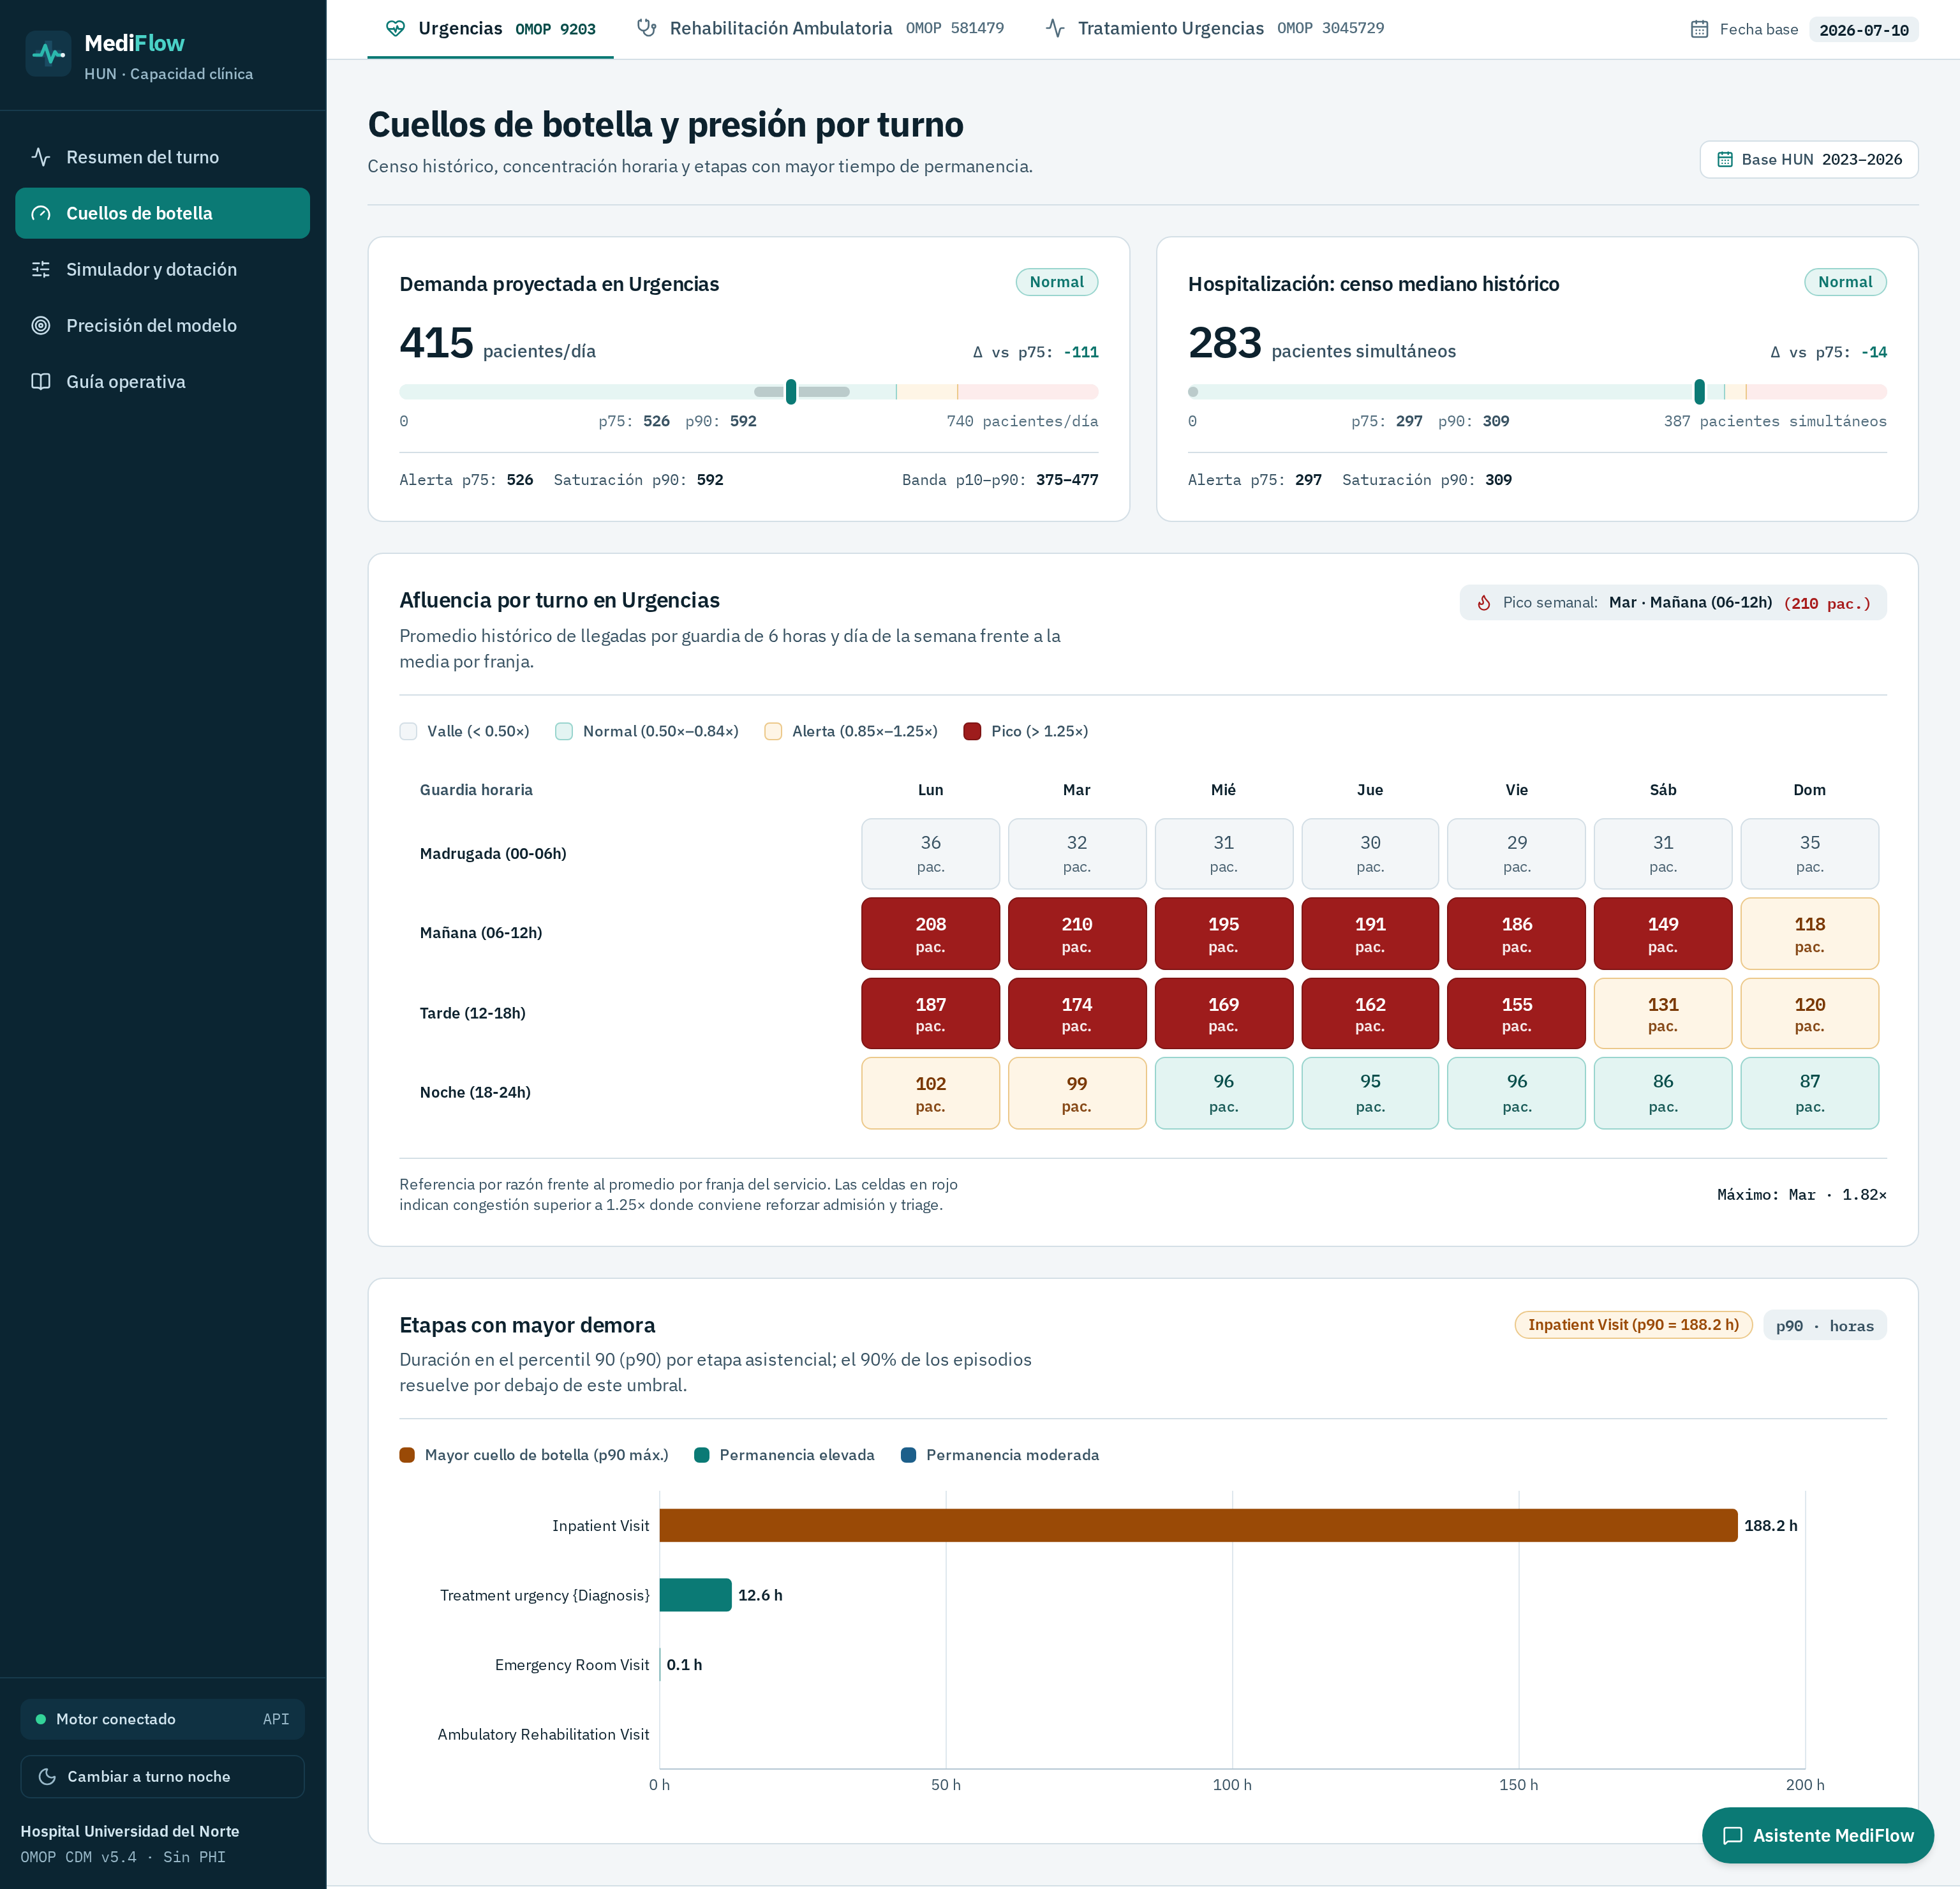
\includegraphics[width=\textwidth,height=0.38\textheight,keepaspectratio]{cuellos_botella.png}
\caption{Vista archivada de cuellos de botella y presión por turno (\protect\nolinkurl{cuellos_botella.png}). No representa ejecución en vivo ni camas habilitadas.}
\label{fig:app_cuellos}
\end{minipage}\hfill
\begin{minipage}[t]{0.48\textwidth}
\centering
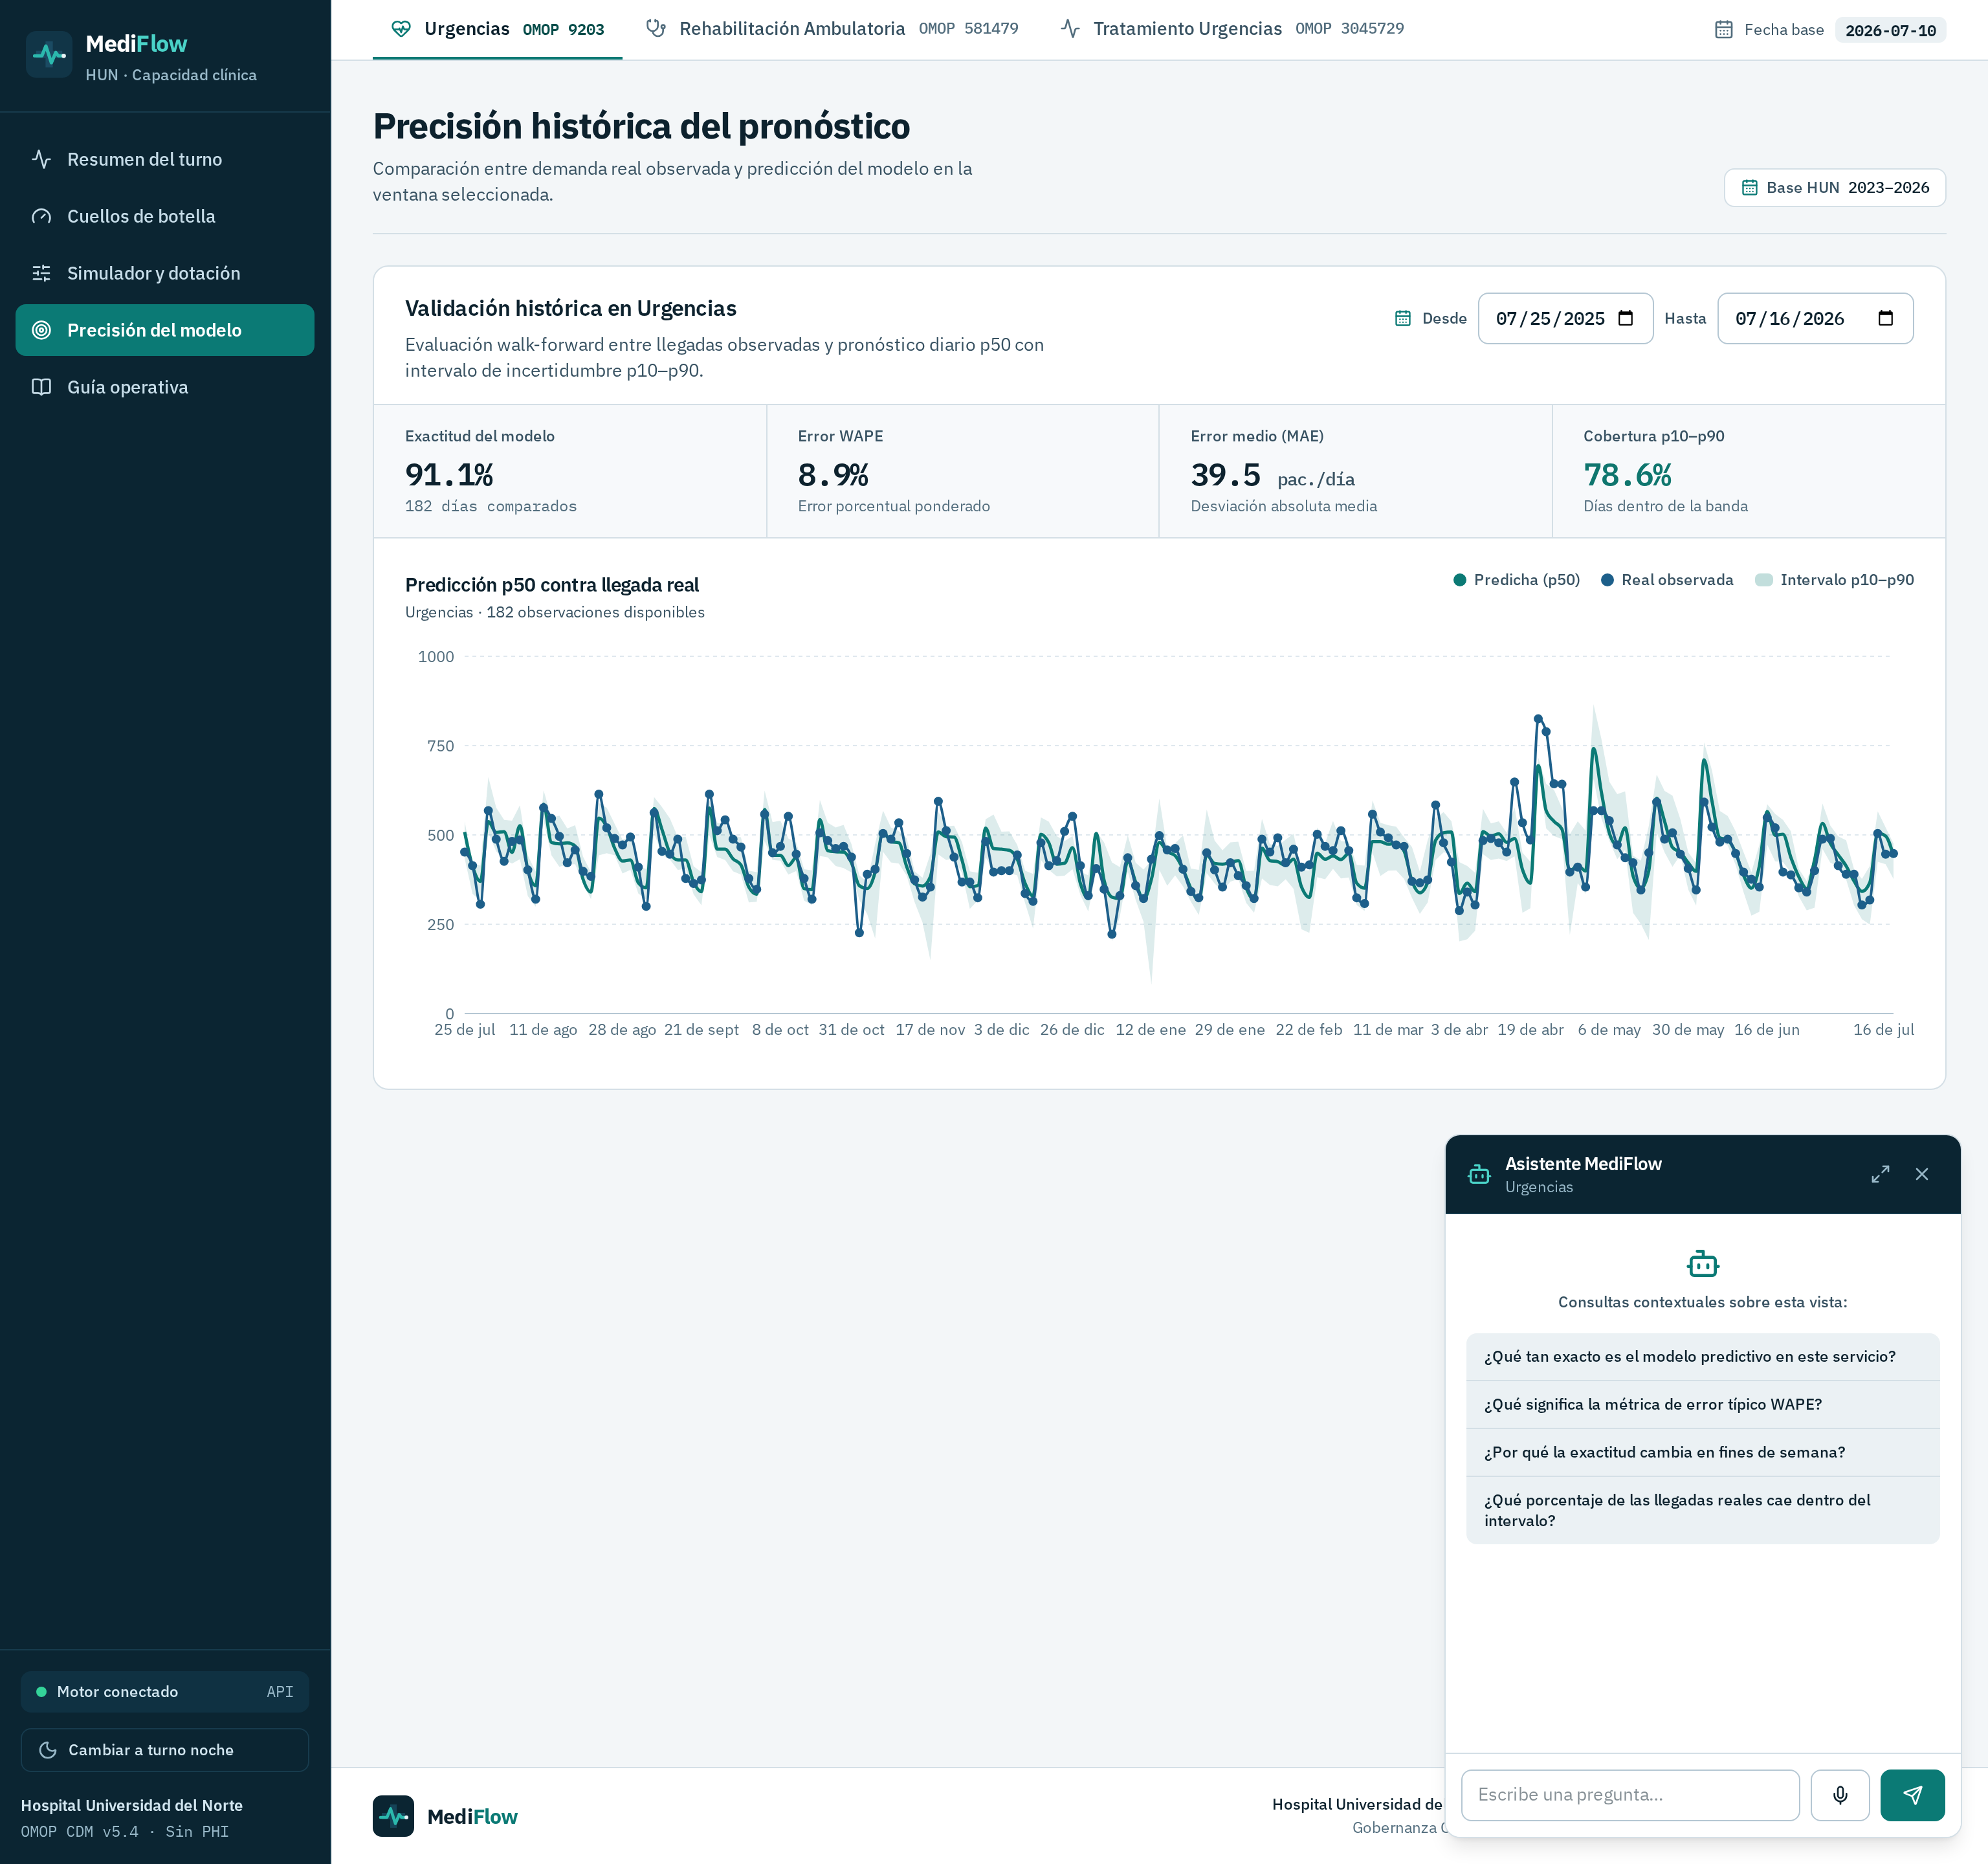
\includegraphics[width=\textwidth,height=0.38\textheight,keepaspectratio]{precision_asistente.png}
\caption{Vista archivada de precisión histórica en Urgencias con asistente (\protect\nolinkurl{precision_asistente.png}). Corresponde al bundle cuantílico \texttt{v2.0} (182\,d).}
\label{fig:app_precision}
\end{minipage}
\end{figure*}

\begin{figure*}[t]
\centering
\begin{minipage}[t]{0.48\textwidth}
\centering
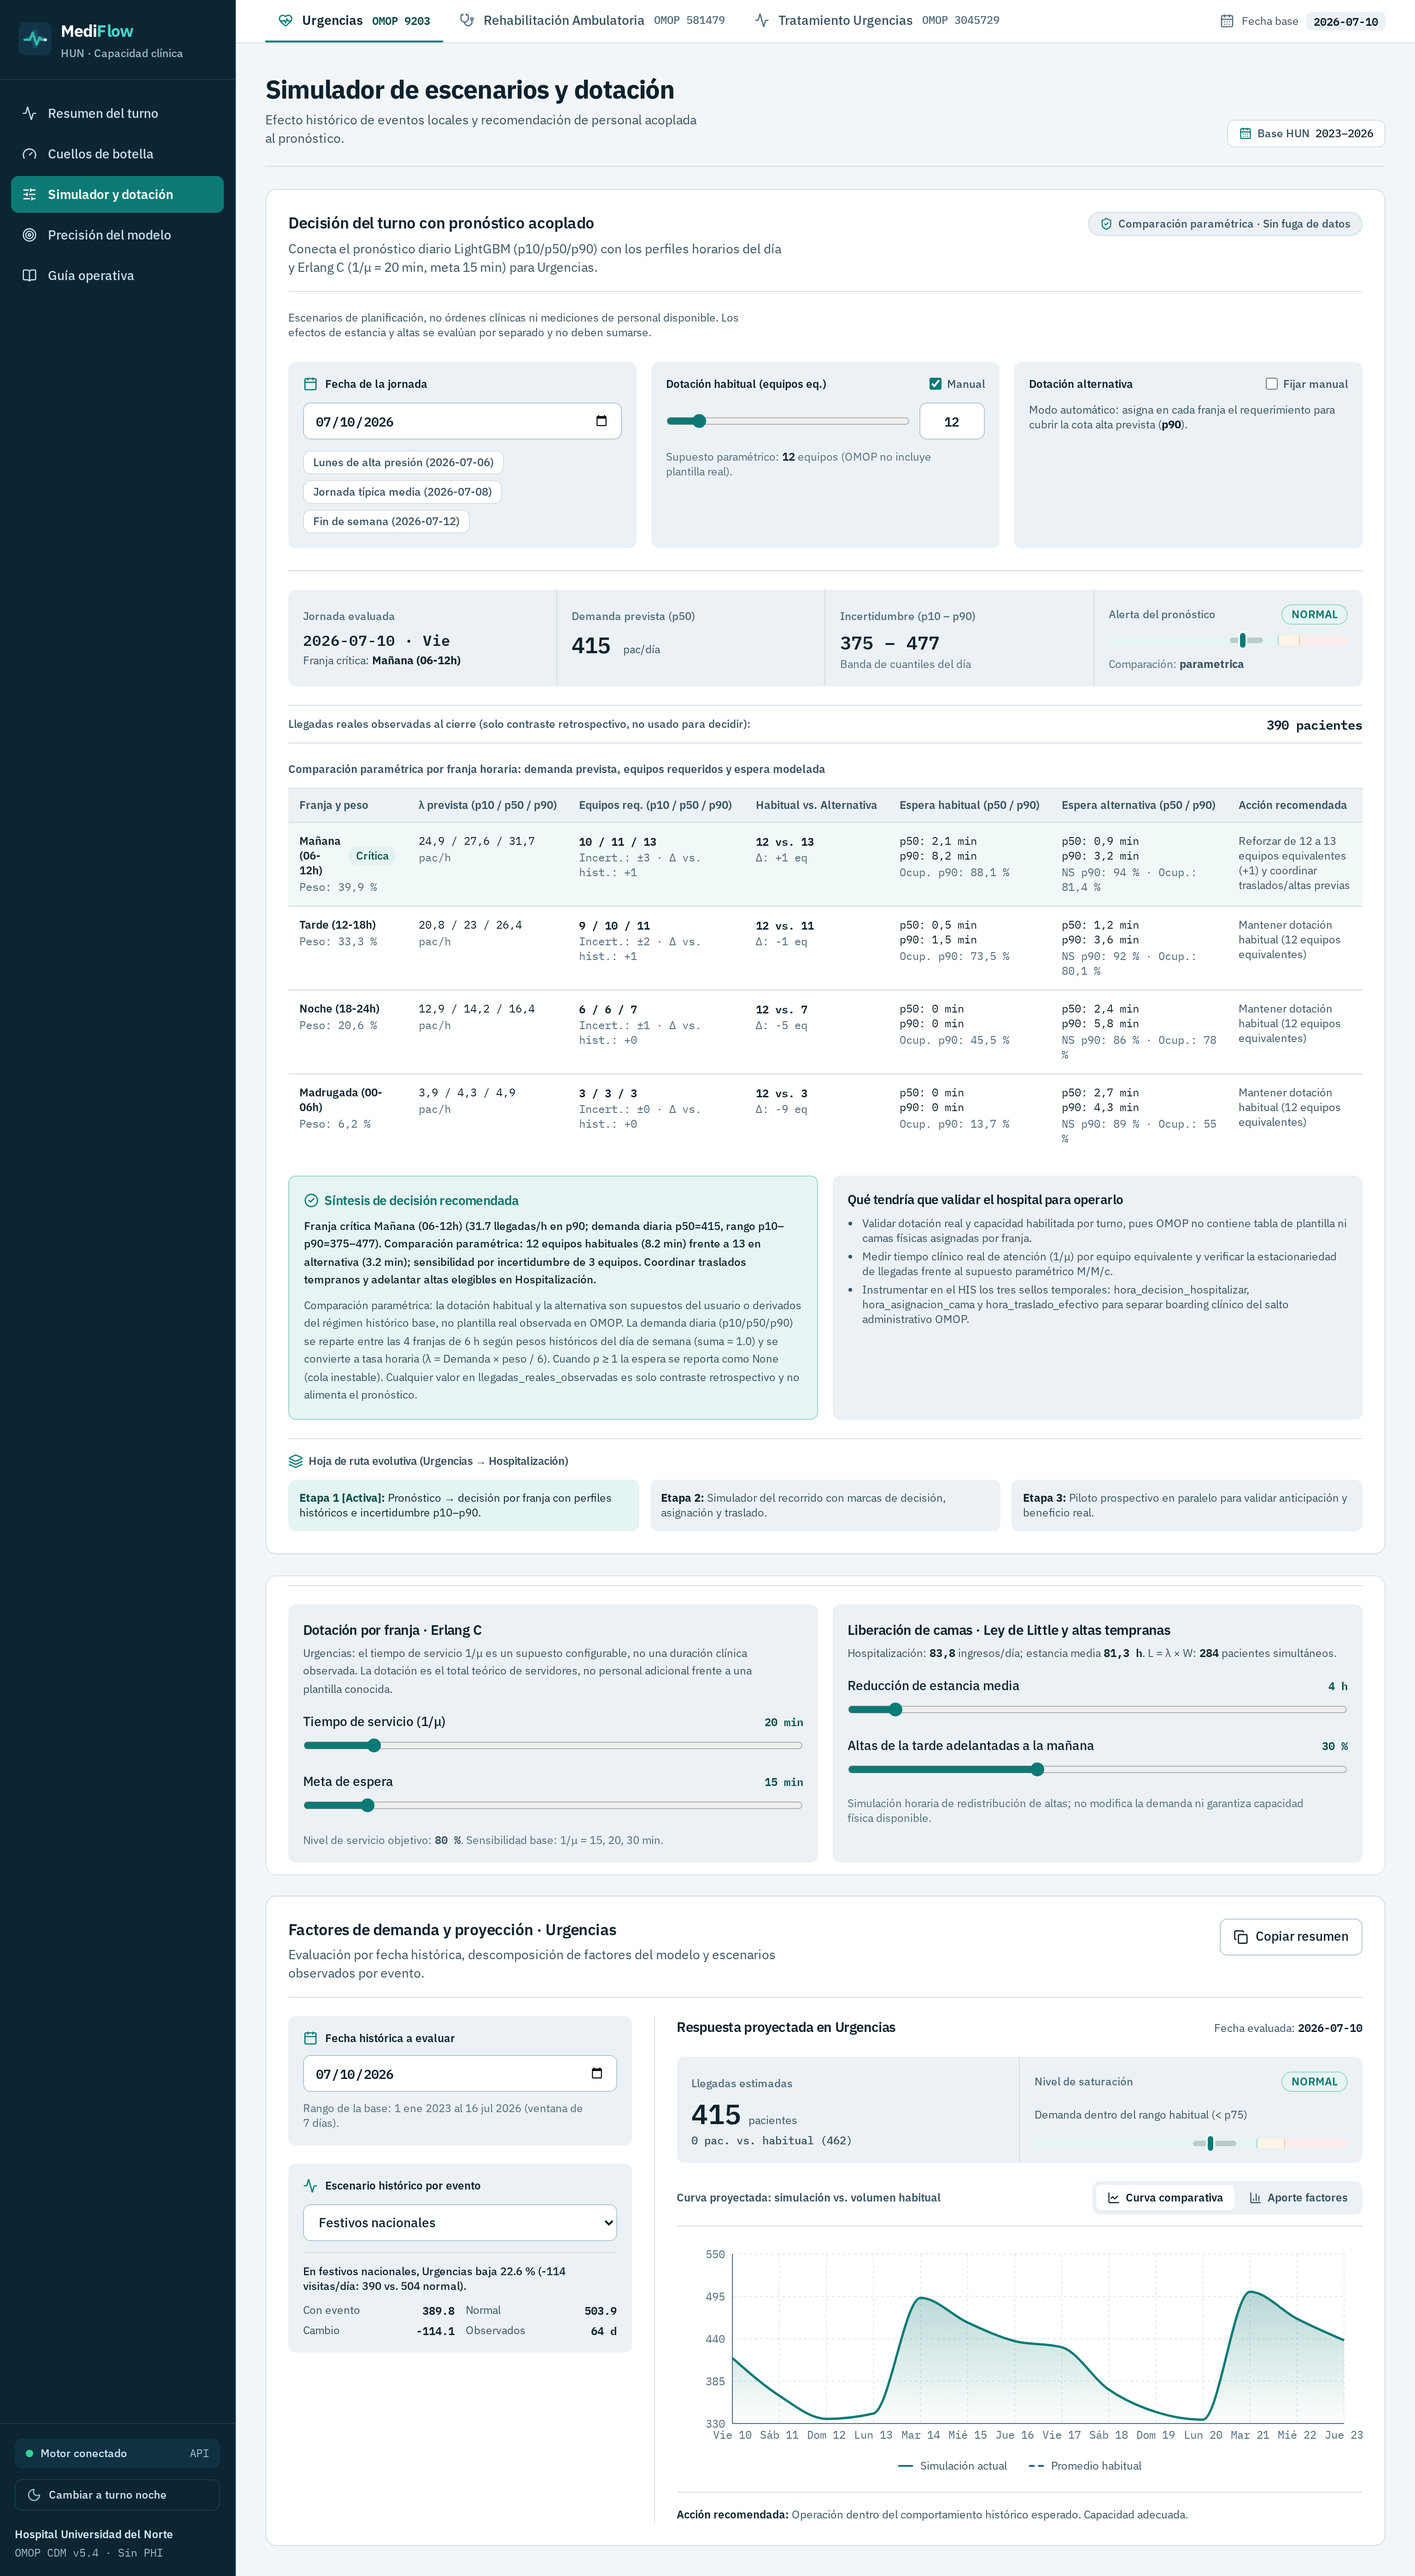
\includegraphics[width=\textwidth,height=0.46\textheight,keepaspectratio]{simulador_optimizacion.png}
\caption{Captura compuesta archivada del simulador (\protect\nolinkurl{simulador_optimizacion.png}). Conserva rótulos previos («Etapa 1 [Activa]», Little 284).}
\label{fig:app_simulador}
\end{minipage}\hfill
\begin{minipage}[t]{0.48\textwidth}
\centering
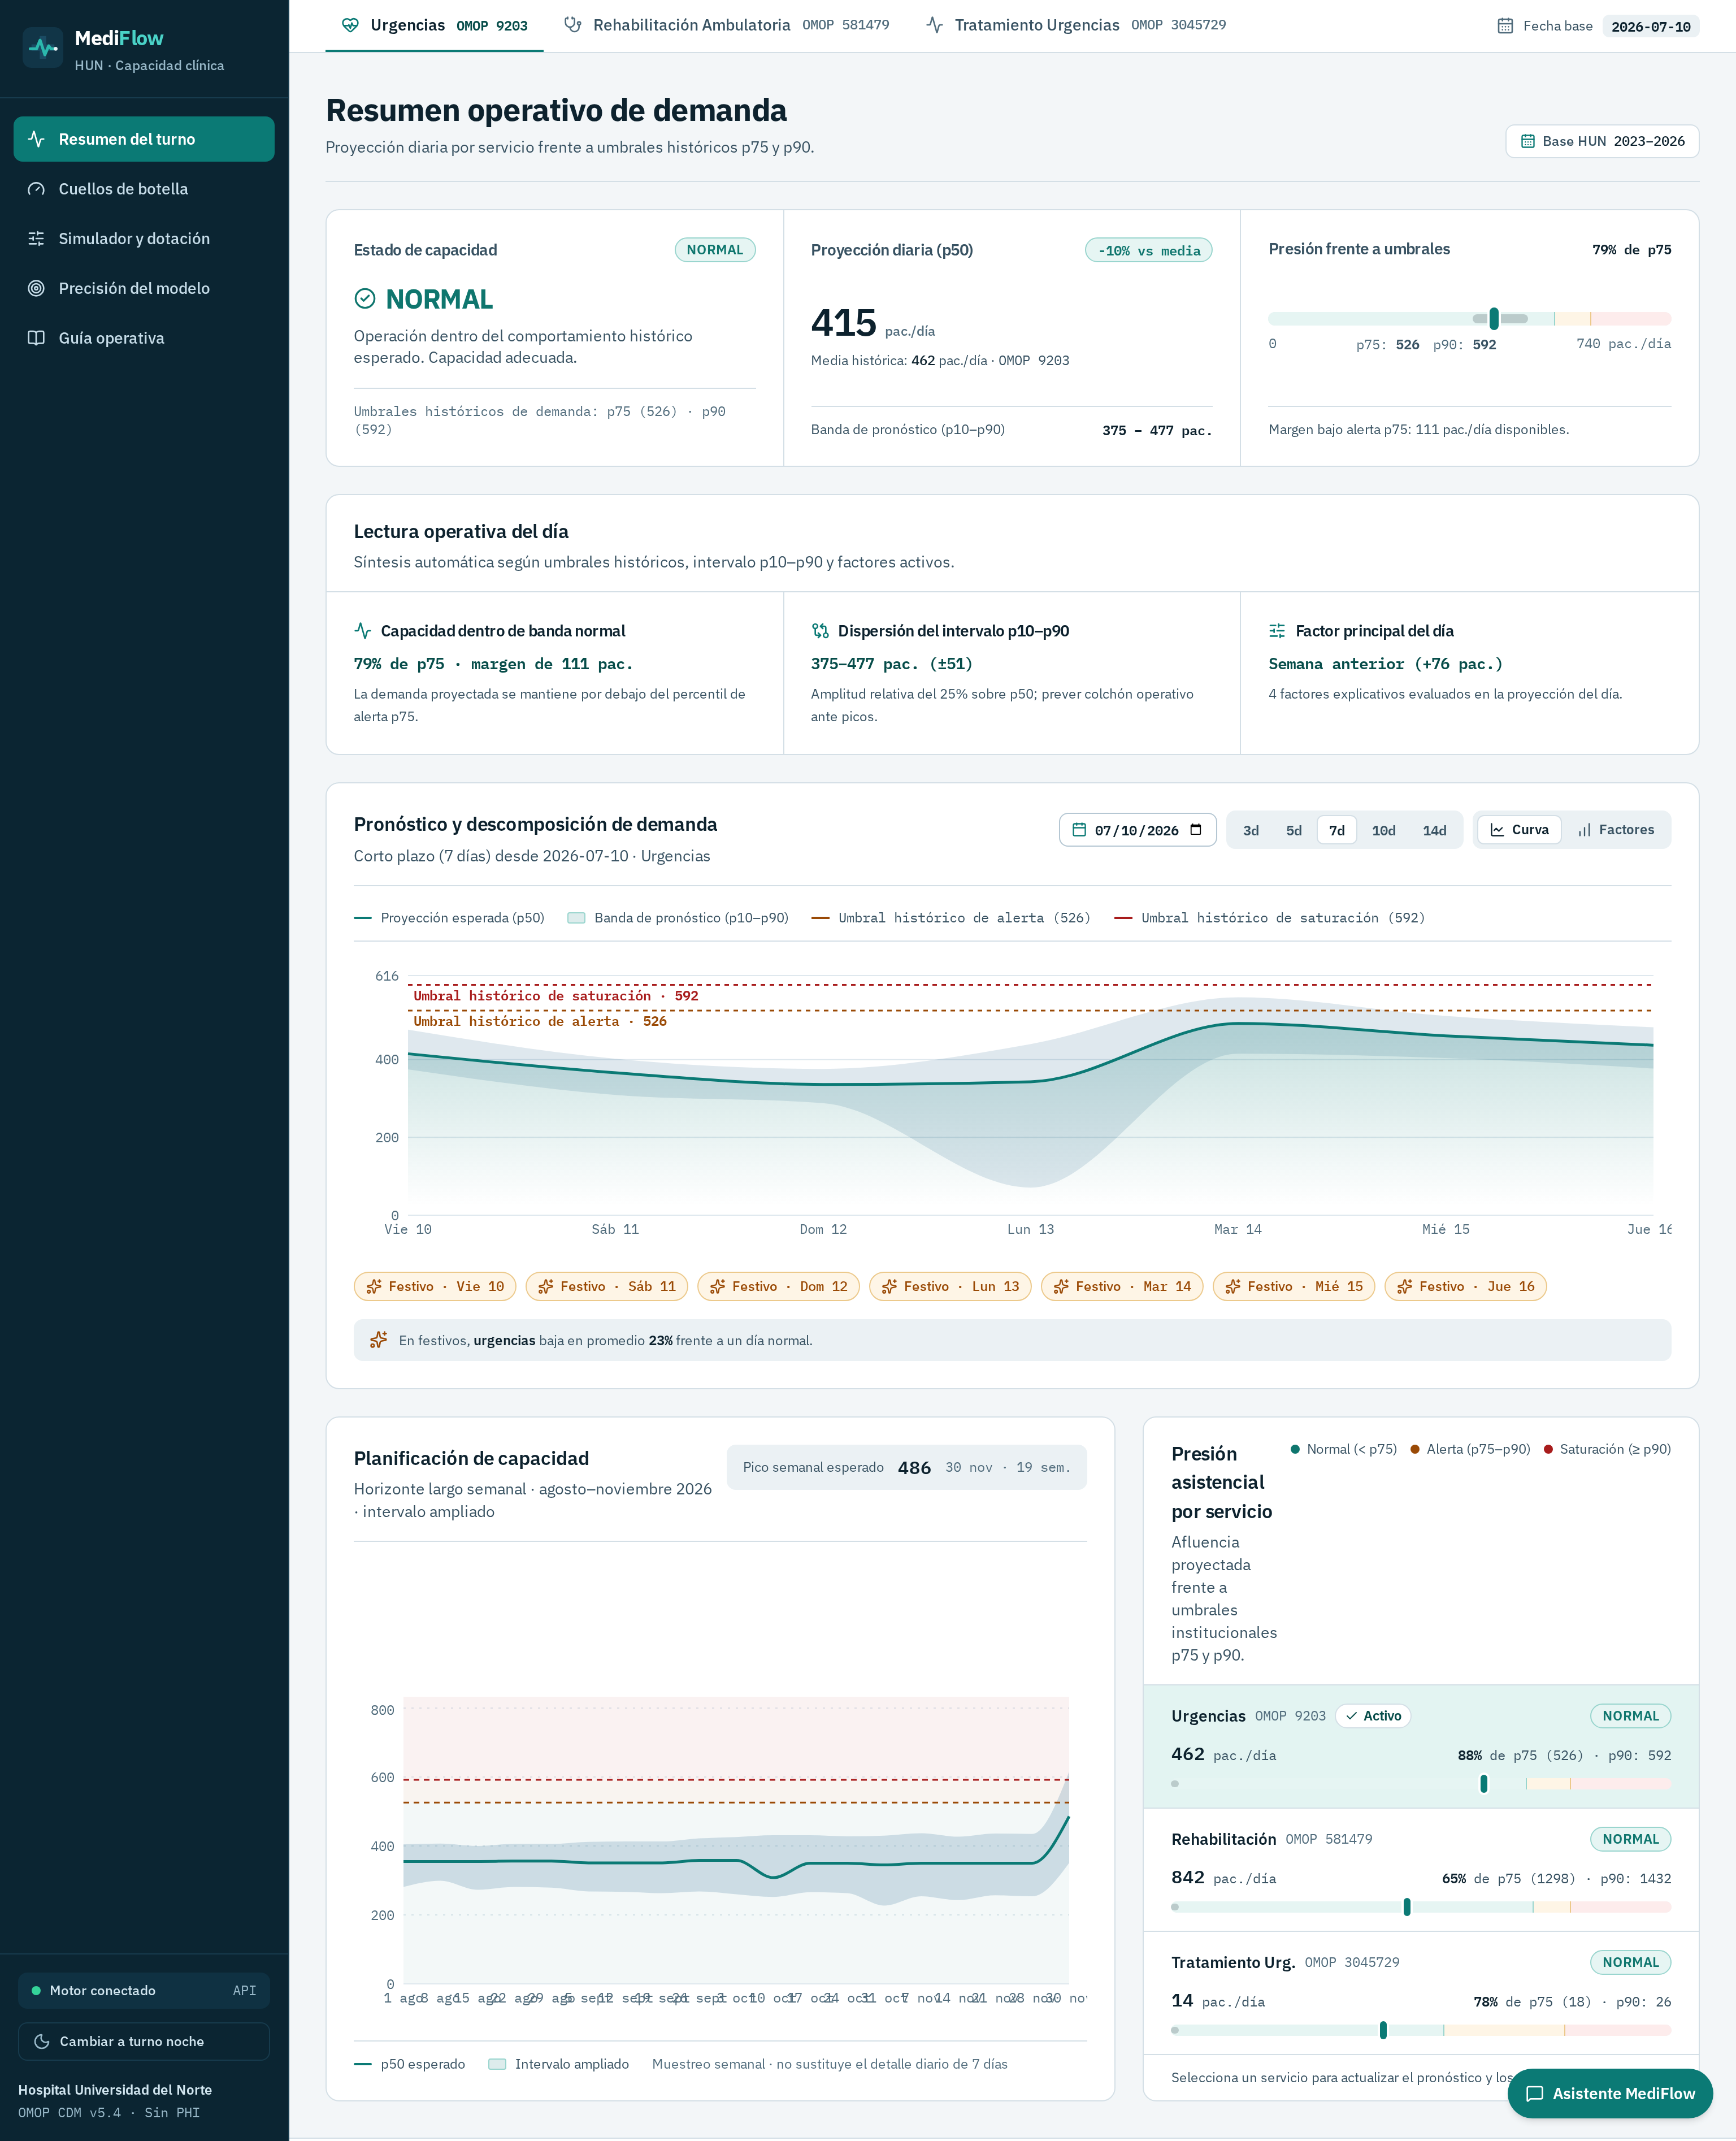
\includegraphics[width=\textwidth,height=0.46\textheight,keepaspectratio]{dashboard_pronostico.png}
\caption{Vista archivada del tablero de pronóstico (\protect\nolinkurl{dashboard_pronostico.png}). Advertencia: rotula «Festivo» del 10 al 16 de julio y superpone ejes.}
\label{fig:app_dashboard}
\end{minipage}
\end{figure*}

\FloatBarrier

% Sección VIII: Ingeniería de software, reproducibilidad y privacidad
% evidencia:E24,E25,E29

\section{Ingeniería de software, reproducibilidad y privacidad}

MediFlow sustenta su confiabilidad técnica en separación modular, trazabilidad de dependencias, pruebas automatizadas y salvaguardas de privacidad~\cite{mediflow2026informe,mediflow2026auditoria}.

\subsection{Estructura real del código y dependencias}

La inspección directa del repositorio verifica la distribución efectiva de responsabilidades:
\begin{itemize}[leftmargin=*,nosep]
\item \textit{Extracción y calidad} (\texttt{src/hun/data/}): \texttt{conexion.py} (solo lectura), \texttt{extraer.py} (mensual resumible), 24 consultas (\texttt{sql/00\_*}--\texttt{23\_*}), \texttt{agregados.py}, \texttt{auditoria.py}, \texttt{conceptos.py} y \texttt{borrar\_datos.py}.
\item \textit{Modelado e inferencia} (\texttt{src/hun/models/}): concentra variables, modelos y reportes en \texttt{validacion.py}, \texttt{linea\_base.py}, \texttt{evaluacion\_factores.py}, \texttt{demanda.py}, \texttt{saturacion.py}, \texttt{explicacion.py}, \texttt{largo\_plazo.py}, \texttt{optimizacion.py}, \texttt{empaquetar.py} y \texttt{predict.py}. En contraste, \texttt{src/hun/features/}, \texttt{visualization/} y \texttt{external/} contienen solo \texttt{\_\_init\_\_.py} documentales (\textit{stubs}) sin lógica implementada.
\item \textit{Factores externos} (\texttt{src/external/}): \texttt{config.py}, \texttt{calendario.py}, \texttt{clima.py}, \texttt{epidemiologia.py} y \texttt{build.py}.
\item \textit{Web y análisis} (\texttt{app/}, \texttt{dashboards/}, \texttt{notebooks/}): FastAPI en \texttt{app/api/\_\_init\_\_.py} y \texttt{chat.py}; frontend React en \texttt{app/src/} (\texttt{OptimizationPanel.jsx}, \texttt{optimizationPayload.test.js}); PBIP y \texttt{preparar\_modelo.py} en \texttt{dashboards/powerbi/}; cuadernos limpios vía \texttt{nbstripout}.
\end{itemize}

Existe una desalineación menor entre manifiestos Python: \texttt{pyproject.toml} (Python $\ge 3{,}11$) declara el núcleo analítico (\texttt{pandas}, \texttt{numpy}, \texttt{scikit-learn}, \texttt{lightgbm}, \texttt{shap}, \texttt{pyarrow}, \texttt{holidays}, \texttt{python-dateutil}, \texttt{matplotlib}, \texttt{seaborn}, \texttt{plotly}, \texttt{requests}, \texttt{python-dotenv}) y extras (\texttt{sqlalchemy>=2.0}, \texttt{psycopg[binary]>=3.1}, \texttt{pytest}, \texttt{ruff}, \texttt{pre-commit}, \texttt{nbstripout}), omitiendo \texttt{fastapi} y \texttt{uvicorn}; \texttt{requirements.txt} sí declara \texttt{fastapi>=0.110.0} y \texttt{uvicorn>=0.28.0}, pero conserva \texttt{streamlit} descartado en \texttt{DEC-006}. En \texttt{app/package.json} constan React \texttt{19.3.1}, Recharts \texttt{3.10.1}, Lucide React \texttt{1.61.0}, Tailwind CSS \texttt{4.3.3} y Vite \texttt{8.3.4}.

\subsection{Evidencia de pruebas y tres niveles de reproducibilidad}

La Tabla~\ref{tab:evidencia_pruebas} separa la verificación local comprobada de las corridas archivadas y de la validación clínica inexistente. Según los insumos disponibles, MediFlow admite tres niveles de reproducción~\cite{mediflow2026informe,mediflow2026auditoria}:
\begin{enumerate}[leftmargin=*,nosep]
\item \textit{Nivel 1 (fixtures sintéticos)}: ejecutable en cualquier clon GitHub sin credenciales mediante \texttt{pytest -q}, \texttt{node --test app/src/lib/optimizationPayload.test.js} y \texttt{npm --prefix app run build}, cubriendo Etapa~1 (\texttt{v2.1}) con datos sintéticos.
\item \textit{Nivel 2 (inferencia estricta con bundle autorizado)}: inicia FastAPI y React leyendo solo \texttt{modelos\_web\_bundle.joblib} con \texttt{HUN\_MODO\_PRODUCCION=1}, sin \texttt{data/}; su distribución requiere autorización institucional.
\item \textit{Nivel 3 (reproducción hospitalaria)}: exige VPN FortiClient, credenciales \texttt{.env} y archivos privados (\texttt{data/raw/*.parquet}, \texttt{data/externos.parquet}) excluidos de Git; no reejecutada para este informe.
\end{enumerate}

\begin{table*}[t]
\caption{Niveles de verificación técnica y estado comprobado en el repositorio (\texttt{803c1a1})}
\label{tab:evidencia_pruebas}
\centering
\footnotesize
\begin{tabularx}{\textwidth}{@{}L{0.21\textwidth} L{0.27\textwidth} L{0.22\textwidth} Y@{}}
\toprule
Evidencia & Alcance verificado & Estado en \texttt{803c1a1} & Qué no acredita \\
\midrule
Recolección estática local (\texttt{pytest}, Node) & 180 pruebas Python en 13 archivos \texttt{test\_*.py} + 3 pruebas Node & Comprobado por recolección (\texttt{--collect-only}) & No equivale a nueva corrida de modelos ni reejecución \\
Cierre de integración (\nolinkurl{cierre_auditoria.md}) & 180/180 Python (211,30\,s; corrida de 228,50\,s en \nolinkurl{tests/README.md}), 3/3 Node, build Vite, Ruff, API sin Parquet & Ejecución previa documentada al integrar \texttt{main} & No prueba calibración sobre BD, eficacia clínica ni despliegue público \\
Validación independiente (\texttt{2026-11-03}) & Revisión interna Sprint 2/3 anti-fuga con 103/103 pruebas & Registro histórico superado por el cierre de 180 pruebas & No es revisión ciega externa ni autorización médica \\
\bottomrule
\end{tabularx}
\ieeenota{Fuentes:~\cite{mediflow2026auditoria},~\cite{mediflow2026validacion} y \texttt{tests/README.md}. Para esta edición editorial no se reejecutó la suite ni se regeneró el archivo \texttt{joblib}.}
\end{table*}

En privacidad, \texttt{conexion.py} fija \texttt{default\_transaction\_read\_only=on}, \texttt{statement\_timeout=120\,s} y filtro sintáctico exclusivo a \texttt{SELECT}/\texttt{WITH}. \texttt{.gitignore} excluye \texttt{data/raw/}, \texttt{data/processed/}, \texttt{.parquet}, \texttt{.env}, \texttt{.pbix} y cachés Power BI, mientras \texttt{borrar\_datos.py} y \texttt{docs/cierre\_datos.md} formalizan el borrado al cierre~\cite{mediflow2026auditoria}. Estos controles no sustituyen la revisión jurídica ni de riesgo de reidentificación por celdas pequeñas en entornos públicos.

% Sección IX: Discusión, recomendaciones accionables y limitaciones
% evidencia:E16,E17,E18,E19,E20,E23,E27

\section{Discusión, recomendaciones accionables y limitaciones}

El valor práctico de MediFlow no reside en automatizar decisiones clínicas, sino en articular datos administrativos heterogéneos bajo criterios auditables, supuestos explícitos y fronteras claras entre versiones.

\subsection{Interpretación operativa e hipótesis alternativas}

Los pronósticos confirman una frontera nítida entre servicios de alto volumen y conteos bajos o intermitentes. En Urgencias (8,4\,\% WAPE en \texttt{lgbm\_final}; 8,91\,\% en bundle \texttt{v2.0}) y Rehabilitación laboral lunes--viernes (85,6\,\%--90,9\,\%), los rezagos semanales y el calendario anticipan oscilaciones y cierres festivos con error acotado. En Tratamiento Urgencias ($\approx 15{,}2$/día; WAPE 43,5\,\% en \texttt{lgbm\_final} y 42,18\,\% en \texttt{v2.0}) y fines de semana de Rehabilitación (51,3\,\% sábado; 15,6\,\% domingo), el error porcentual combina denominador pequeño con deriva semanal bajo el techo Poisson idealizado (77,0\,\% semanal observado frente a 92,3\,\% teórico)~\cite{mediflow2026demanda}; conviene planificar sobre MAE ($\approx 6{,}4$--$6{,}6$/día) y agregados semanales.

En congestión hospitalaria, la consistencia matemática de Ley de Little en población común (\num{277,52} frente a \num{277,47} pacientes medios) convive con dos matices críticos~\cite{mediflow2026informe}: (1) la correlación ecológica negativa ($r = -0{,}481$) entre censo mensual de Hospitalización y $p_{90}$ ponderado de transición Tratamiento Urgencias $\rightarrow$ Hospitalización (\num{25,13}\,h en meses normales vs. \num{23,70}\,h en censo alto) descarta atribuir las demoras registradas directamente a saturación de piso sin auditar cierres tardíos o solapamientos~\cite{mediflow2026optimizacion}; y (2) adelantar el 35\,\% de altas vespertinas recorta horas rojas de 9,32\,\% a 6,26\,\% ($-32{,}8\,\%$ rel.; $-3{,}06$\,pp) sin alterar el pico máximo de 359 pacientes.

\subsection{Estado consolidado de capacidades y recomendaciones}

La Tabla~\ref{tab:estado_capacidades} delimita código implementado, estado en el artefacto \texttt{v2.0}/PBIP y pendientes al corte \texttt{803c1a1}. La Tabla~\ref{tab:recomendaciones} sintetiza las recomendaciones condicionadas \texttt{REC-01} a \texttt{REC-05}~\cite{mediflow2026optimizacion,mediflow2026informe}; no implican metas aprobadas ni ahorro garantizado. La hoja de ruta contempla: (1) completar el paquete \texttt{v2.1} autorizado con perfiles por corte, Little alineado y cuantiles recalibrados; (2) desarrollar el simulador de recorrido (Etapa~2) con camas, dotación, tiempos reales y tres sellos HIS (\texttt{hora\_\allowbreak decision\_\allowbreak hospitalizar}, \texttt{hora\_\allowbreak asignacion\_\allowbreak cama}, \texttt{hora\_\allowbreak traslado\_\allowbreak efectivo}); y (3) ejecutar un piloto prospectivo en modo sombra (Etapa~3).

\begin{table*}[t]
\caption{Estado verificado de capacidades entre código, artefacto servido (\texttt{v2.0}) / PBIP y pendientes}
\label{tab:estado_capacidades}
\centering
\footnotesize
\begin{tabularx}{\textwidth}{@{}L{0.21\textwidth} L{0.25\textwidth} L{0.24\textwidth} Y@{}}
\toprule
Capacidad o módulo & Implementación en código & Estado en bundle \texttt{v2.0} / PBIP & Trabajo pendiente \\
\midrule
Pronóstico puntual 1--7\,d (\texttt{lgbm\_final}) & Implementado en \texttt{demanda.py} con nivel local y recencia & No es el modelo servido; reporte del \texttt{2026-11-18} & Evaluar nivel local en familia cuantílica \\
Pronóstico cuantílico web ($p_{10}/p_{50}/p_{90}$ + SHAP) & Implementado en \texttt{explicacion.py} y \texttt{predict.py} & Activo en \texttt{v2.0} (corte \texttt{2026-07-17}) & Recalibrar cobertura (64,3\,\%--78,6\,\%) e incluir Carnaval/Sem. Santa \\
Largo plazo a 120 días & Implementado en \texttt{largo\_plazo.py} ($p_{05}/p_{95}$ ensanchado) & Activo en \texttt{/api/largo-plazo} (corrida \texttt{v2.0}) & Reconciliar reporte \texttt{2026-11-03} vs. bundle \\
Erlang~C, Little y altas tempranas & Implementado en \texttt{optimizacion.py} (interpolación API) & Activo en \texttt{v2.0} con Little híbrido (\num{284,01}) & Regenerar con Little alineado (\num{277,52}) y medir $1/\mu$ real \\
Acoplamiento por corte Etapa~1 & Implementado en \texttt{empaquetar.py} (\texttt{v2.1}) + fixtures & Ausente en \texttt{v2.0}: \texttt{disponible: false} & Regenerar \texttt{v2.1} autorizado con \texttt{perfiles\_horarios} \\
Asistente \texttt{/api/chat} & 6 herramientas + respaldo offline (\texttt{chat.py}) & Operativo contra salidas del bundle & Validar \textit{end-to-end} con clave autorizada \\
Tablero Power BI (PBIP) & 7 pág., 12 tab., 18 rel., 43 DAX (\texttt{2026-04-30}) & Definiciones locales corregidas; sin datos & Revisar en Desktop, alinear cortes y republicar \\
Simulador Etapa~2 y piloto Etapa~3 & Diseño conceptual en \texttt{informe\_final.md} & No implementado ni validado en clínica & Instrumentar 3 marcas HIS, capacidad y piloto sombra \\
\bottomrule
\end{tabularx}
\ieeenota{Consolidación desde~\cite{mediflow2026auditoria},~\cite{mediflow2026bundle},~\cite{mediflow2026pbip} e inspección de \texttt{src/hun/models/} y \texttt{app/}.}
\end{table*}

\begin{table*}[t]
\caption{Recomendaciones operacionales condicionadas (\texttt{REC-01} a \texttt{REC-05}) y criterios de validación}
\label{tab:recomendaciones}
\centering
\footnotesize
\begin{tabularx}{\textwidth}{@{}l L{0.23\textwidth} L{0.31\textwidth} Y@{}}
\toprule
ID & Acción propuesta & Resultado modelado o archivado & Condición e indicador de piloto \\
\midrule
\texttt{REC-01} & Validar equipos en Urgencias (06--12\,h) & Demanda $p_{90}$ (39,67/h): 15 eq. vs. 12 norm.; esp. 6,09\,min & Medir duración real vs. supuesto 20\,min y plantilla por turno \\
\texttt{REC-02} & Revisar capacidad en Rehab. (06--12\,h) & Demanda $p_{90}$ (133,33/h): 70 eq. vs. 42 norm.; esp. 5,30\,min & Contrastar agenda, atención supuesta (30\,min) y puestos \\
\texttt{REC-03} & Investigar demoras de estancia en Hosp. & $-4$\,h libera 13,97 camas eq. (4,92\,\% de Little híbrido) & Auditar demoras administrativas preservando alta clínica \\
\texttt{REC-04} & Pilotar egreso seguro intradía & Adelantar 35\,\% [14,20)$\rightarrow$[08,12): rojas 9,32\,\%$\rightarrow$6,26\,\% (pico 359) & Evaluar en piloto con umbral $>309$, reingreso y seguridad \\
\texttt{REC-05} & Auditar sellos Trat. Urg. $\rightarrow$ Hosp. & \num{47670} pasos; $p_{90}$ pond. 24,45\,h; $r = -0{,}481$ con censo & Instrumentar decisión, asignación y traslado en HIS \\
\bottomrule
\end{tabularx}
\ieeenota{Propuestas tomadas de~\cite{mediflow2026optimizacion} y~\cite{mediflow2026informe}; no implican calendario ni compromiso institucional aprobado.}
\end{table*}

\subsection{Limitaciones consolidadas}

Seis límites acotan el uso actual: (a) ausencia en OMOP de camas físicas, personal y tiempos clínicos reales; (b) carácter estadístico del filtro $p_{99{,}9}$ y exclusión de diagnósticos/procedimientos/laboratorio como predictores; (c) ambigüedad administrativa de \texttt{espera\_h} con solapamientos negativos; (d) cobertura cuantílica de \texttt{v2.0} inferior al 80\,\% nominal y ausencia de \texttt{perfiles\_horarios}; (e) divergencia de cortes entre Power BI (abril 2026 sin republicación verificada) y demanda (julio 2026), y entre corridas de largo plazo; y (f) ausencia de validación prospectiva en vivo o autorización clínica.

% Sección X: Conclusiones y trabajo futuro

\section{Conclusiones y trabajo futuro}

MediFlow aporta una base analítica reproducible e interpretable para estudiar la demanda y la presión operativa del Hospital Universidad del Norte sobre agregados OMOP CDM v5.4, integrando reconstrucción de flujo, predicción con validación temporal estricta y simulaciones paramétricas bajo supuestos explícitos. En el corte documental del repositorio (\texttt{803c1a1}), el contraste riguroso entre fuentes confirma que el experimento puntual \texttt{lgbm\_final} reduce el WAPE diario global de 18,0\,\% a 10,5\,\% (mejora relativa archivada de 41,6\,\%) con sólido desempeño en Urgencias (8,4\,\%) y Rehabilitación laboral, mientras el artefacto cuantílico servido (\texttt{v2.0}) registra WAPE de 8,91\,\%, 11,08\,\% y 42,18\,\% por servicio con coberturas de 78,57\,\%, 64,29\,\% y 73,08\,\% en 182 días. En Hospitalización, el balance documentado con $N_0=0$ en 12 cortes y la concordancia de Ley de Little sobre población común (\num{277,52} frente a \num{277,47} pacientes medios) respaldan la consistencia censal tras el filtro $p_{99{,}9}$, en tanto adelantar el 35\,\% de altas vespertinas proyecta una reducción relativa de 32,8\,\% en horas rojas (9,32\,\% a 6,26\,\%) manteniendo el pico en 359 pacientes.

Estos hallazgos retrospectivos justifican una validación operativa supervisada, pero no demuestran beneficio clínico ni sustituyen mediciones físicas del hospital. Quedan cinco prioridades inmediatas: (1) regenerar el paquete web hacia \texttt{v2.1} sobre agregados autorizados habilitando \texttt{perfiles\_horarios} reales y Ley de Little alineada; (2) recalibrar cuantiles incorporando \texttt{carnaval\_y\_semana\_santa} y nivel local en el bundle, reconciliando además las métricas de largo plazo; (3) abrir, validar visualmente y republicar el tablero Power BI (PBIP) aclarando la brecha abril--julio 2026; (4) auditar los sellos de transición e instrumentar las tres marcas HIS junto con capacidad instalada y tiempos reales de atención; y (5) ejecutar un piloto en modo sombra y aplicar el borrado seguro de datos locales al término del certamen.


\FloatBarrier

\printbibliography[title={Referencias}]

\appendices
% Anexos técnicos y de trazabilidad (A, B, C y D)

\section{Trazabilidad de evidencias, discrepancias resueltas y conversión editorial}
\label{app:trazabilidad}

Las Tablas~\ref{tab:anexo_matriz_a} y~\ref{tab:anexo_matriz_b} consolidan las 29 unidades de evidencia (\texttt{E01}--\texttt{E29}) que rigen el contrato numérico de este informe.

\begin{table*}[t]
\caption{Matriz de evidencias (\texttt{E01}--\texttt{E15}) y límites de interpretación}
\label{tab:anexo_matriz_a}
\centering
\scriptsize
\begin{tabularx}{\textwidth}{@{}L{0.04\textwidth} L{0.27\textwidth} L{0.24\textwidth} L{0.15\textwidth} Y@{}}
\toprule
ID & Tema y cifra principal & Fuente del repositorio & Tipo de evidencia & Límite obligatorio \\
\midrule
E01 & Rúbrica 15/15/20/20/15/5/10\,\% y entregables & T\&C p.~4 \S\S13--14; Enunc. p.~3 & Norma oficial & No derivar requisitos del informe del equipo \\
E02 & Desempates: optimización $\rightarrow$ rigor $\rightarrow$ flujo & T\&C p.~5 \S16 & Norma oficial & No inventar reglas adicionales \\
E03 & Corte demanda: \texttt{2026-07-16} (excl. \texttt{2026-07-17}) & \nolinkurl{docs/inventario_base.md} & Resultado archivado & No unificar con corte Power BI abril 2026 \\
E04 & Deduplicación: \num{228259} copias (13,38\,\%) de \num{1706001} & \nolinkurl{docs/calidad_datos.md} & Resultado archivado & No extrapolar 13,38\,\% a etapas (\texttt{visit\_detail}) \\
E05 & Limpieza $p_{99{,}9}$ y \texttt{LEFT JOIN} huérfanas & \nolinkurl{16_duracion_etapas_diaria.sql} & Implementación SQL & Prevalece sobre texto previo de \nolinkurl{calidad_datos.md} \\
E06 & Censo y stock $N_0=0$ en 12 cortes & \nolinkurl{reports/informe_final.md} \S3 & Verificación BD doc. & No reejecutada contra PostgreSQL aquí \\
E07 & Presión: Hosp. 283/297/309; Trat. 201/239/272 & \nolinkurl{docs/resultados/saturacion.md} & Resultado archivado & Pacientes concurrentes, no camas habilitadas \\
E08 & Escalera Poisson: 26 pl., 18,0$\rightarrow$15,6$\rightarrow$10,5\,\% (41,6\,\%) & \nolinkurl{docs/resultados/modelo_demanda.md} & Resultado archivado & Experimento Poisson; mejoras pre-redondeo \\
E09 & Poisson por servicio: 8,4 / 11,0 / 43,5\,\% WAPE & \nolinkurl{docs/resultados/modelo_demanda.md} & Resultado archivado & No transferir al modelo cuantílico web \\
E10 & Externos: acepta festivos y Carnaval/Sem. Santa & \nolinkurl{docs/resultados/factores_externos.md} & Resultado archivado & Sin números de clima/epi en tabla actual \\
E11 & Anti-fuga: enmascarar $y$ desde origen y lag $\ge 7$\,d & \nolinkurl{src/hun/models/demanda.py} & Implementación & No acredita ausencia de fuga en retrospectivo \\
E12 & Intervalos 3-nov: 83,2\,\% global (85,2/72,0/75,8\,\%) & \nolinkurl{docs/resultados/intervalos_shap.md} & Corrida previa (3-nov) & Incluye \texttt{Otros}; no valida bundle \texttt{v2.0} \\
E13 & Bundle \texttt{v2.0}: 8,91/11,08/42,18\,\%, cob. 78,57/64,29/73,08\,\% & \nolinkurl{models/modelos_web_bundle.joblib} & Metadatos inspecc. & 182\,d; no reejecutado ni igual a E08 \\
E14 & Largo plazo: 13 pl. 120\,d; 15,7\,\% (3-nov) y \texttt{v2.0} & \nolinkurl{largo_plazo.md} y bundle \texttt{v2.0} & Corrida arch. / bundle & Pliegues solapados; bandas base $p_{05}/p_{95}$ \\
E15 & Erlang~C: Urg. 15 eq. (39,67/h); Reh. 70 eq. (133,33/h) & \nolinkurl{docs/resultados/optimizacion.md} & Escenario archivado & Equipos equivalentes; $1/\mu$ supuesto \\
\bottomrule
\end{tabularx}
\ieeenota{Adaptado de \texttt{reports/preparacion\_latex/02\_MATRIZ\_EVIDENCIAS.md} sobre el commit \nolinkurl{803c1a1f866a978cce8b4622269ccfb4749ba59e}.}
\end{table*}

\begin{table*}[t]
\caption{Matriz de evidencias (\texttt{E16}--\texttt{E29}) y límites de interpretación}
\label{tab:anexo_matriz_b}
\centering
\scriptsize
\begin{tabularx}{\textwidth}{@{}L{0.04\textwidth} L{0.27\textwidth} L{0.24\textwidth} L{0.15\textwidth} Y@{}}
\toprule
ID & Tema y cifra principal & Fuente del repositorio & Tipo de evidencia & Límite obligatorio \\
\midrule
E16 & Little alineado: \num{277,52} vs. media \num{277,47} (1.294\,d) & \nolinkurl{reports/informe_final.md} \S3 & Verificación BD doc. & Mediana 283 no se contrasta contra Little \\
E17 & Little bundle \texttt{v2.0}: \num{284,01} ($W=81{,}297$\,h); $-4$\,h $\rightarrow$ 13,97 & \nolinkurl{models/modelos_web_bundle.joblib} & Metadatos inspecc. & Población híbrida; no es expansión física \\
E18 & Altas 35\,\%: rojas 9,32\,\%$\rightarrow$6,26\,\% ($-32{,}8\,\%$ rel.); pico 359 & \nolinkurl{docs/resultados/optimizacion.md} & Simulación histórica & Altas fraccionales; $-3{,}06$\,pp; no clínico \\
E19 & Transiciones: \num{47670} pasos; $p_{90}$ pond. 24,45\,h; $r=-0{,}481$ & \nolinkurl{docs/resultados/optimizacion.md} & Resultado archivado & No $p_{90}$ global ni prueba causal de cama \\
E20 & Modo por corte: código \texttt{v2.1}; \texttt{v2.0} sin perfiles & \nolinkurl{src/hun/models/predict.py} & Código y bundle & Probado solo en fixtures; \texttt{disponible: false} \\
E21 & Interfaz selector modo y referencia en panel & \nolinkurl{OptimizationPanel.jsx} & Implementación & Build pasado; no prueba despliegue público \\
E22 & \texttt{/api/modelo}, 15 rutas reales, HTTP 503 en fallo & \nolinkurl{app/api/__init__.py} & Implementación & Sin \texttt{/api/salud}; CORS $\ne$ autenticación \\
E23 & Power BI: 12 tab., 18 rel., 43 DAX, 7 pág., corte \texttt{2026-04-30} & \nolinkurl{model.bim} y \nolinkurl{pages.json} & Definición PBIP & Ediciones locales no prueban republicación \\
E24 & Pruebas: 180 Python (211,30\,s / 228,50\,s) + 3 Node & \nolinkurl{docs/cierre_auditoria.md} & Ejecución previa & Solo recolección verificada en \texttt{803c1a1} \\
E25 & Validación histórica 3-nov: 103 pruebas & \nolinkurl{validacion_independiente.md} & Registro histórico & Sin revisión ciega ni autorización clínica \\
E26 & Fuentes externas al \texttt{2026-10-27} (clima a \texttt{2026-10-21}) & \nolinkurl{data/externos_fuentes.json} & Registro archivado & No garantiza completitud diaria ni aceptación \\
E27 & Recomendaciones \texttt{REC-01} a \texttt{REC-05} & \nolinkurl{reports/informe_final.md} & Propuestas doc. & Condicionadas; sin metas aprobadas ni piloto \\
E28 & Cuatro capturas PNG y GIF de interfaz & \nolinkurl{README.md} y \nolinkurl{docs/img/app/} & Evidencia archivada & Captura simulador compuesta; notas de versión \\
E29 & Privacidad: solo lectura SQL, exclusiones Git & \nolinkurl{src/hun/data/conexion.py} & Control implementado & No sustituye auditoría legal ni celdas pequeñas \\
\bottomrule
\end{tabularx}
\ieeenota{Continuación de la Tabla~\ref{tab:anexo_matriz_a}.}
\end{table*}

\subsection{Inconsistencias documentales resueltas y cambio editorial}

Al contrastar el repositorio se resolvieron nueve inconsistencias: (1) separación entre largo plazo del 3 de noviembre~\cite{mediflow2026largoplazo} y corrida empaquetada en \texttt{v2.0}; (2) detección de que \texttt{v2.0} omite \texttt{init\_score}, pesos de recencia y \texttt{carnaval\_y\_semana\_santa}; (3) exclusión de \texttt{04\_censo\_etapas.png} previa al filtro $p_{99{,}9}$; (4) advertencia sobre festivos repetidos del 10 al 16 de julio en \texttt{dashboard\_pronostico.png}; (5) inclusión de \texttt{GET /api/parametros} entre las 15 rutas reales y obsolescencia de rutas en \texttt{DEC-007} y \texttt{tests/README.md}; (6) fecha correcta de \texttt{saturacion.md} (\texttt{2026-11-19}) y ancla desactualizada en \texttt{informe\_final.md} \S5.5; (7) dos duraciones para las 180 pruebas Python (211,30\,s vs. 228,50\,s) y desfase tras PR~\#12 en \texttt{cierre\_auditoria.md}; (8) identificación de \texttt{features/}, \texttt{visualization/} y \texttt{external/} bajo \texttt{src/hun/} como \textit{stubs} vacíos y desfase \texttt{pyproject.toml}/\texttt{requirements.txt}; y (9) discrepancia entre \texttt{dashboards/README.md} (mayo incompleto) e \texttt{inventario\_base.md} (sin meses vacíos hasta junio).

Editorialmente, esta edición convierte el informe original APA~7 (61 páginas) a formato de conferencia IEEE (\texttt{IEEEtran} a dos columnas, citas numéricas y bibliografía \texttt{biblatex-ieee}), omitiendo las dos entradas bibliográficas exclusivas de guía APA y preservando intactos título, autores, omisión de docente/tutor/asignatura y todo el contenido sustantivo.

\FloatBarrier

\section{Tablas extensas de backtest, horizonte, Erlang~C y balance}
\label{app:tablas_extensas}

Las Tablas~\ref{tab:anexo_pliegues}--\ref{tab:anexo_cortes_n0} preservan las series completas de los 26 pliegues, el desglose por día del horizonte, la proyección mensual agosto--noviembre, las 12 franjas de Erlang~C y los 12 cortes de balance horario en Hospitalización.

\begin{table*}[t]
\caption{Estabilidad temporal por pliegue del experimento puntual (26 pliegues \textit{walk-forward})}
\label{tab:anexo_pliegues}
\centering
\scriptsize
\begin{tabularx}{\textwidth}{@{}r c r r r | r c r r r@{}}
\toprule
Pliegue & Origen & WAPE Base & WAPE \texttt{lgbm\_final} & Dif. (pp) & Pliegue & Origen & WAPE Base & WAPE \texttt{lgbm\_final} & Dif. (pp) \\
\midrule
0 & \texttt{2025-07-25} & 7,8\,\% & 8,2\,\% & $+0{,}4$ & 13 & \texttt{2026-01-23} & 13,0\,\% & 12,0\,\% & $-1{,}0$ \\
1 & \texttt{2025-08-08} & 8,9\,\% & 8,4\,\% & $-0{,}5$ & 14 & \texttt{2026-02-06} & 12,5\,\% & 10,0\,\% & $-2{,}5$ \\
2 & \texttt{2025-08-22} & 8,2\,\% & 8,5\,\% & $+0{,}3$ & 15 & \texttt{2026-02-20} & 15,0\,\% & 9,2\,\% & $-5{,}8$ \\
3 & \texttt{2025-09-05} & 9,5\,\% & 8,8\,\% & $-0{,}7$ & 16 & \texttt{2026-03-06} & 7,0\,\% & 6,4\,\% & $-0{,}6$ \\
4 & \texttt{2025-09-19} & 6,8\,\% & 9,9\,\% & $+3{,}1$ & 17 & \texttt{2026-03-20} & 23,9\,\% & 5,4\,\% & $-18{,}5$ \\
5 & \texttt{2025-10-03} & 8,4\,\% & 7,5\,\% & $-0{,}9$ & 18 & \texttt{2026-04-03} & 23,8\,\% & 11,5\,\% & $-12{,}3$ \\
6 & \texttt{2025-10-17} & 6,3\,\% & 6,4\,\% & $+0{,}1$ & 19 & \texttt{2026-04-17} & 33,0\,\% & 27,6\,\% & $-5{,}4$ \\
7 & \texttt{2025-10-31} & 25,2\,\% & 8,2\,\% & $-17{,}0$ & 20 & \texttt{2026-05-01} & 24,1\,\% & 12,6\,\% & $-11{,}5$ \\
8 & \texttt{2025-11-14} & 22,7\,\% & 5,8\,\% & $-16{,}9$ & 21 & \texttt{2026-05-15} & 21,7\,\% & 7,0\,\% & $-14{,}7$ \\
9 & \texttt{2025-11-28} & 9,8\,\% & 11,0\,\% & $+1{,}2$ & 22 & \texttt{2026-05-29} & 7,4\,\% & 7,5\,\% & $+0{,}1$ \\
10 & \texttt{2025-12-12} & 11,5\,\% & 9,2\,\% & $-2{,}3$ & 23 & \texttt{2026-06-12} & 26,8\,\% & 8,9\,\% & $-17{,}9$ \\
11 & \texttt{2025-12-26} & 137,9\,\% & 28,0\,\% & $-109{,}9$ & 24 & \texttt{2026-06-26} & 27,2\,\% & 10,3\,\% & $-16{,}9$ \\
12 & \texttt{2026-01-09} & 28,9\,\% & 17,6\,\% & $-11{,}3$ & 25 & \texttt{2026-07-10} & 17,5\,\% & 11,2\,\% & $-6{,}3$ \\
\bottomrule
\end{tabularx}
\ieeenota{Tomado de~\cite{mediflow2026demanda} (sec.~5, 18 de noviembre de 2026). Diferencia en pp = \texttt{lgbm\_final} menos línea base.}
\end{table*}

\begin{table*}[t]
\caption{Desempeño por día del horizonte y exactitud ($1-\text{WAPE}$) por servicio en \texttt{lgbm\_final}}
\label{tab:anexo_horizonte}
\centering
\scriptsize
\begin{tabularx}{\textwidth}{@{}Y r r r r r r r r@{}}
\toprule
Métrica / Servicio & 1 (vie) & 2 (sáb) & 3 (dom) & 4 (lun) & 5 (mar) & 6 (mié) & 7 (jue) & Total \\
\midrule
WAPE agregado & 10,3\,\% & 17,0\,\% & 10,2\,\% & 12,4\,\% & 9,5\,\% & 9,6\,\% & 9,4\,\% & 10,5\,\% \\
MAE agregado (pac.) & 53,34 & 27,39 & 12,11 & 55,73 & 55,28 & 57,04 & 53,73 & 44,94 \\
Sesgo agregado (pac.) & $-4{,}20$ & $-4{,}86$ & $-2{,}47$ & $-3{,}97$ & $-6{,}59$ & $-9{,}71$ & $-8{,}06$ & $-5{,}70$ \\
\midrule
Urgencias ($1-\text{WAPE}$) & 91,7\,\% & 91,9\,\% & 91,6\,\% & 91,7\,\% & 91,3\,\% & 92,4\,\% & 90,9\,\% & 91,6\,\% \\
Urgencias (prom. real/d) & 441,5 & 379,8 & 344,2 & 496,8 & 504,7 & 469,0 & 466,0 & 443,16 \\
Rehabilitación ($1-\text{WAPE}$) & 89,4\,\% & 51,3\,\% & 15,6\,\% & 85,6\,\% & 90,6\,\% & 90,0\,\% & 90,9\,\% & 89,0\,\% \\
Rehabilitación (prom./d) & \num{1095,3} & 87,1 & 2,2 & 835,7 & \num{1219,5} & \num{1306,2} & \num{1239,8} & 826,54 \\
Tratamiento ($1-\text{WAPE}$) & 56,8\,\% & 48,1\,\% & 44,2\,\% & 63,0\,\% & 54,6\,\% & 68,5\,\% & 56,8\,\% & 56,5\,\% \\
Tratamiento (prom./d) & 15,8 & 17,4 & 10,0 & 15,1 & 17,0 & 16,3 & 14,4 & 15,17 \\
\bottomrule
\end{tabularx}
\ieeenota{Fuente:~\cite{mediflow2026demanda} (secs. 2, 3 y 3.1). Todos los orígenes caen en viernes, confundiendo día de horizonte y día de semana.}
\end{table*}

\begin{table*}[t]
\caption{Proyección mensual agosto--noviembre de 2026: reporte histórico frente a bundle servido \texttt{v2.0}}
\label{tab:anexo_lp_mensual}
\centering
\scriptsize
\begin{tabularx}{\textwidth}{@{}Y c r L{0.22\textwidth} r L{0.22\textwidth}@{}}
\toprule
Servicio & Mes & \multicolumn{2}{c}{Reporte \texttt{2026-11-03} (prom./d, banda y total)} & \multicolumn{2}{c}{Bundle \texttt{v2.0} (prom./d, banda y total)} \\
\midrule
Urgencias (\texttt{9203}) & \texttt{2026-08} & 215,7 & [173,9; 254,6] $\cdot$ \num{6686} & 422,0 & [343,8; 487,5] $\cdot$ \num{13082} \\
 & \texttt{2026-09} & 221,0 & [182,3; 263,0] $\cdot$ \num{6631} & 433,2 & [352,6; 510,6] $\cdot$ \num{12995} \\
 & \texttt{2026-10} & 217,1 & [170,6; 261,0] $\cdot$ \num{6731} & 421,5 & [337,4; 506,4] $\cdot$ \num{13066} \\
 & \texttt{2026-11} & 216,0 & [159,6; 268,9] $\cdot$ \num{6479} & 415,6 & [318,2; 511,9] $\cdot$ \num{12467} \\
\midrule
Rehabilitación (\texttt{581479}) & \texttt{2026-08} & 333,6 & [76,9; 514,5] $\cdot$ \num{10340} & 661,5 & [171,0; 789,3] $\cdot$ \num{20507} \\
 & \texttt{2026-09} & 385,9 & [60,4; 554,8] $\cdot$ \num{11577} & 789,6 & [150,4; 932,3] $\cdot$ \num{23689} \\
 & \texttt{2026-10} & 351,4 & [31,0; 550,0] $\cdot$ \num{10894} & 727,5 & [98,4; 877,4] $\cdot$ \num{22553} \\
 & \texttt{2026-11} & 330,5 & [6,6; 619,9] $\cdot$ \num{9915} & 677,4 & [38,6; 843,7] $\cdot$ \num{20321} \\
\midrule
Tratamiento Urg. (\texttt{3045729}) & \texttt{2026-08} & 8,4 & [2,4; 46,7] $\cdot$ 262 & 15,6 & [3,0; 34,3] $\cdot$ 485 \\
 & \texttt{2026-09} & 8,5 & [0,6; 48,8] $\cdot$ 255 & 16,1 & [0,9; 36,1] $\cdot$ 482 \\
 & \texttt{2026-10} & 8,5 & [1,0; 51,5] $\cdot$ 263 & 15,9 & [2,3; 38,7] $\cdot$ 494 \\
 & \texttt{2026-11} & 8,4 & [1,4; 59,0] $\cdot$ 253 & 15,7 & [1,7; 39,9] $\cdot$ 470 \\
\bottomrule
\end{tabularx}
\ieeenota{Comparación entre~\cite{mediflow2026largoplazo} y~\cite{mediflow2026bundle}; extrapolaciones desde el corte julio de 2026, no demanda real observada.}
\end{table*}

\begin{table*}[t]
\caption{Dimensionamiento Erlang~C completo por servicio y franja de seis horas}
\label{tab:anexo_erlang_12}
\centering
\scriptsize
\begin{tabularx}{\textwidth}{@{}L{0.21\textwidth} Y r r r r r r r@{}}
\toprule
Servicio ($1/\mu$) & Franja & $\lambda_{\text{norm}}$ & $\lambda_{p75}$ & $\lambda_{p90}$ & $c_{\text{norm}}$ & $c_{p75}$ & $c_{p90}$ & Esp. $p_{90}$ (min) \\
\midrule
Urgencias (20\,min) & Mañana (06--12\,h) & 29,250 & 35,333 & 39,667 & 12 & 14 & 15 & 6,094 \\
 & Tarde (12--18\,h) & 25,593 & 30,333 & 34,333 & 10 & 12 & 13 & 7,265 \\
 & Noche (18--24\,h) & 15,392 & 17,667 & 20,367 & 7 & 8 & 9 & 3,062 \\
 & Madrug. (00--06\,h) & 5,236 & 6,333 & 7,500 & 3 & 4 & 4 & 4,265 \\
\midrule
Rehabilitación (30\,min) & Mañana (06--12\,h) & 77,584 & 118,667 & 133,333 & 42 & 62 & 70 & 5,303 \\
 & Tarde (12--18\,h) & 58,174 & 95,667 & 108,000 & 32 & 51 & 57 & 5,905 \\
 & Noche (18--24\,h) & 1,442 & 2,333 & 3,333 & 2 & 3 & 3 & 6,745 \\
 & Madrug. (00--06\,h) & 0,255 & 0,333 & 0,667 & 1 & 1 & 2 & 0,857 \\
\midrule
Trat. Urg. (20\,min) & Mañana (06--12\,h) & 0,415 & 0,667 & 1,000 & 1 & 1 & 2 & 0,571 \\
 & Tarde (12--18\,h) & 0,682 & 1,000 & 1,333 & 1 & 2 & 2 & 1,039 \\
 & Noche (18--24\,h) & 0,819 & 1,000 & 1,667 & 1 & 2 & 2 & 1,672 \\
 & Madrug. (00--06\,h) & 0,338 & 0,667 & 1,000 & 1 & 1 & 2 & 0,571 \\
\bottomrule
\end{tabularx}
\ieeenota{Fuente:~\cite{mediflow2026optimizacion}. Tasas $\lambda$ en llegadas/h; la última columna indica la espera media bajo demanda $p_{90}$.}
\end{table*}

\begin{table*}[t]
\caption{Balance horario archivado en 12 cortes PostgreSQL para Hospitalización (\texttt{9201}, regla común $p_{99{,}9}$)}
\label{tab:anexo_cortes_n0}
\centering
\scriptsize
\begin{tabularx}{\textwidth}{@{}Y r r r r r@{}}
\toprule
Corte horario $t$ & Entradas $E$ & Salidas $S$ & $N_0 + E - S$ & Conteo directo & Dif. \\
\midrule
\texttt{2023-01-01 00:00} (stock inicial) & 0 & 0 & 0 & 0 & 0 \\
\texttt{2023-01-01 04:00} & 3 & 0 & 3 & 3 & 0 \\
\texttt{2023-01-01 15:00} & 15 & 1 & 14 & 14 & 0 \\
\texttt{2023-01-02 00:00} & 37 & 2 & 35 & 35 & 0 \\
\texttt{2023-01-03 00:00} & 120 & 27 & 93 & 93 & 0 \\
\texttt{2023-01-25 04:00} (tras calentamiento) & \num{2232} & \num{1959} & 273 & 273 & 0 \\
\texttt{2024-06-15 12:00} & \num{44576} & \num{44282} & 294 & 294 & 0 \\
\texttt{2025-12-01 18:00} & \num{91583} & \num{91304} & 279 & 279 & 0 \\
\texttt{2026-07-17 07:00} (última entrada) & \num{108494} & \num{108178} & 316 & 316 & 0 \\
\texttt{2026-07-18 00:00} (cierre día 1.294) & \num{108494} & \num{108216} & 278 & 278 & 0 \\
\texttt{2026-07-18 05:00} & \num{108494} & \num{108216} & 278 & 278 & 0 \\
\texttt{2026-07-18 06:00} (última salida) & \num{108494} & \num{108494} & 0 & 0 & 0 \\
\bottomrule
\end{tabularx}
\ieeenota{Verificación documentada en~\cite{mediflow2026informe} (sec.~3, \num{108494} etapas con filtro \num{1176,3}\,h y 91 huérfanas). En las cuatro variantes del equipo resultó $N_0=0$ y diferencia 0 (incluyendo la cohorte bruta de \num{108601} etapas).}
\end{table*}

\section{Contratos HTTP, consultas SQL y modelo semántico Power BI}
\label{app:contratos_sql_pbip}

Las Tablas~\ref{tab:anexo_endpoints} y~\ref{tab:anexo_sql_pbip} inventarían las 15 rutas HTTP vigentes en FastAPI, las 24 consultas SQL agregadas y la estructura semántica del tablero PBIP.

\begin{table*}[t]
\caption{Inventario completo de los 15 endpoints HTTP implementados en FastAPI}
\label{tab:anexo_endpoints}
\centering
\scriptsize
\begin{tabularx}{\textwidth}{@{}l L{0.28\textwidth} L{0.27\textwidth} Y@{}}
\toprule
Método & Ruta HTTP & Función invocada & Contrato y alcance \\
\midrule
\texttt{GET} & \texttt{/api/health} & \texttt{health} & Estado del servicio (\texttt{HUN}, \texttt{1.0.0}) \\
\texttt{GET} & \texttt{/api/modelo} & \texttt{obtener\_estado\_modelo} & Versión, SHA-256, corte, métricas \texttt{v2.0}, perfiles \\
\texttt{GET} & \texttt{/api/servicios} & \texttt{obtener\_servicios} & Catálogo con \texttt{mediaDiaria}, $p_{75}$, $p_{90}$ \\
\texttt{GET} & \texttt{/api/parametros} & \texttt{obtener\_parametros} & Parámetros, mapeo OMOP y rango de fechas \\
\texttt{GET} & \texttt{/api/turnos/\{servicio\}} & \texttt{obtener\_turnos\_reales} & Matriz $4\times 7$ de afluencia por franja y día \\
\texttt{GET} & \texttt{/api/ocupacion} & \texttt{obtener\_ocupacion\_real} & Demanda diaria relativa a $p_{75}/p_{90}$ (no camas) \\
\texttt{GET} & \texttt{/api/cuellos-botella} & \nolinkurl{obtener_indicadores_cuellos_botella} & Duración ($p_{50}$, $p_{90}$, $p_{99}$) y umbrales de censo \\
\texttt{GET} & \texttt{/api/comparacion/\{servicio\}} & \nolinkurl{obtener_comparacion_real} & Serie \textit{walk-forward} de 182\,d y exactitud \\
\texttt{GET} & \texttt{/api/efectos-eventos/\{servicio\}} & \nolinkurl{obtener_efectos_eventos} & Variación histórica observada por tipo de evento \\
\texttt{GET} & \texttt{/api/largo-plazo/\{servicio\}} & \nolinkurl{obtener_pronostico_largo_plazo} & Backtest 120\,d y serie ago--nov 2026 del bundle \\
\texttt{GET} & \texttt{/api/optimizacion} & \texttt{obtener\_optimizacion} & Erlang~C, Little, altas, transición y \texttt{REC-01..05} \\
\texttt{POST} & \texttt{/api/predecir} & \texttt{predecir} & Mediana $p_{50}$, $[p_{10}, p_{90}]$, alerta y top-5 SHAP \\
\texttt{POST} & \texttt{/api/predecir-rango} & \texttt{predecir\_rango} & Serie 1--30\,d (no implica backtest a 30\,d) \\
\texttt{POST} & \texttt{/api/optimizacion/simular} & \texttt{simular\_optimizacion} & Parámetros Erlang/Little/altas y \texttt{modo\_demanda} \\
\texttt{POST} & \texttt{/api/chat} & \texttt{endpoint\_chat} & 6 herramientas de solo lectura y respaldo offline \\
\bottomrule
\end{tabularx}
\ieeenota{Verificado en \texttt{app/api/\_\_init\_\_.py} y \texttt{app/api/chat.py}. \texttt{/api/optimizacion/simular} admite \texttt{tiempo\_servicio\_min} (5--120), \texttt{meta\_espera\_min} (1--120), \texttt{reduccion\_estancia\_horas} (0--48), \texttt{pct\_altas\_tempranas} (0--80), \texttt{modo\_demanda} (\texttt{historico} o \texttt{pronostico}), \texttt{fecha}, \texttt{dotacion\_habitual}, \texttt{dotacion\_alternativa} y \texttt{dotacion\_referencia}.}
\end{table*}

\begin{table*}[t]
\caption{Catálogo resumido de las 24 consultas SQL agregadas y del modelo semántico PBIP}
\label{tab:anexo_sql_pbip}
\centering
\scriptsize
\begin{tabularx}{\textwidth}{@{}L{0.24\textwidth} Y@{}}
\toprule
Componente & Inventario verificado en archivos fuente \\
\midrule
SQL inventario (\texttt{00}--\texttt{03}, \texttt{06}) & \texttt{00\_tablas\_tamano}, \texttt{01\_cobertura\_mensual}, \texttt{02\_tipos\_visita}, \texttt{03\_tipos\_etapa}, \texttt{06\_precision\_horas} \\
SQL flujo (\texttt{04}--\texttt{05}) & \texttt{04\_entradas\_por\_hora} (\texttt{COUNT(DISTINCT ...)}), \texttt{05\_salidas\_por\_hora} \\
SQL auditoría (\texttt{07}--\texttt{12}) & \texttt{07\_auditoria\_nulos}, \texttt{08\_auditoria\_duplicados}, \texttt{09\_auditoria\_etapas}, \texttt{10\_auditoria\_personas}, \texttt{11\_auditoria\_llegadas\_diarias}, \texttt{12\_auditoria\_etapas\_diarias} \\
SQL agregados (\texttt{13}--\texttt{18}, \texttt{23}) & \texttt{13\_llegadas\_diarias\_perfil}, \texttt{14\_etapas\_entradas\_por\_hora} ($p_{99{,}9}$), \texttt{15\_etapas\_salidas\_por\_hora} ($p_{99{,}9}$), \texttt{16\_duracion\_etapas\_diaria} ($p_{99{,}9}$, \texttt{LEFT JOIN}), \texttt{17\_duracion\_etapas\_por\_franja}, \texttt{18\_transiciones\_etapas}, \texttt{23\_duracion\_etapas\_percentiles} (sin recorte) \\
SQL conceptos (\texttt{19}--\texttt{22}) & \texttt{19\_conceptos\_visitas}, \texttt{20\_conceptos\_diagnosticos}, \texttt{21\_conceptos\_procedimientos}, \texttt{22\_conceptos\_mediciones} \\
\midrule
PBIP tablas (12) y relaciones (18) & 5 dimensiones (\texttt{dim\_etapa}, \texttt{dim\_fecha}, \texttt{dim\_hora}, \texttt{dim\_servicio}, \texttt{dim\_sexo}), 6 hechos (\texttt{fact\_censo\_etapa\_hora}, \texttt{fact\_duracion\_diaria}, \texttt{fact\_duracion\_franja}, \texttt{fact\_llegadas\_hora}, \texttt{fact\_llegadas\_perfil}, \texttt{fact\_transiciones}) y \texttt{\_Medidas} \\
PBIP medidas DAX (43) y páginas (7) & Censo/semáforo (17), entradas/salidas/flujo (3), llegadas/perfil (8), duraciones (6), transiciones (4) y resumen (5); páginas: Inicio, 1.~Resumen ejecutivo, 2.~Saturación por área, 3.~Esperas y flujo, 4.~Demanda, 5.~Hallazgos y recomendaciones, 6.~Metodología y glosario; parámetros \texttt{RutaDatos} y \texttt{FechaCorte = 2026-04-30} \\
\bottomrule
\end{tabularx}
\ieeenota{Fuentes: \texttt{src/hun/data/extraer.py}, \texttt{src/hun/data/sql/}, \texttt{model.bim} y \texttt{pages.json} en \texttt{dashboards/powerbi/HUN\_CuellosBotella/}.}
\end{table*}

\FloatBarrier

\raggedbottom
\section{Comandos de reproducción y verificación local}
\label{app:comandos}

Los comandos siguientes documentan la verificación local y el despliegue estricto sin carpetas privadas; la regeneración de reportes requiere agregados autorizados~\cite{mediflow2026informe,mediflow2026auditoria}:
{\scriptsize
\begin{verbatim}
# 1. Suite automatizada y build frontend
pytest -q
node --test app/src/lib/optimizationPayload.test.js
npm --prefix app run build

# 2. API en modo estricto (solo artefacto)
HUN_MODO_PRODUCCION=1 \
HUN_BUNDLE_PATH=models/modelos_web_bundle.joblib \
ALLOWED_ORIGINS=https://mediflow.example.org \
  uvicorn app.api:app --host 0.0.0.0 --port 8000

# 3. Regeneracion (requiere data/raw/ autorizado)
python -m hun.models.demanda
python -m hun.models.saturacion
python -m hun.models.explicacion
python -m hun.models.largo_plazo
python -m hun.models.optimizacion
python -m hun.models.empaquetar

# 4. Simulacion de borrado seguro al cierre
python -m hun.data.borrar_datos
\end{verbatim}
}


\end{document}
